%!TEX root = ../PhD_thesis__Lilian_Besson

% ----------------------------------------------------------------------
\chapter{More Efficient Spectrum Usage of IoT Networks with Selfish MAB Learning}
\label{chapter:4}
\minitoc
% ----------------------------------------------------------------------

In this Chapter~\ref{chapter:4}, we present two models of Internet of Things networks, composed of many independent devices that are able to run MAB algorithm to learn and improve their access to the network.
The two models are presented mathematically, and numerical simulations justify the interest of the proposed algorithms.
We also present a proof-of-concept real-world validation of the advantage of using Multi-Armed Bandit algorithms for the first model, by showing and explaining a demonstration implemented on USRP \cite{USRPDocumentation} cards.

More precisely, on the one hand, we start by presenting in Section~\ref{sec:4:firstModel} a model where independent devices use an IoT network composed of different channels, used by static devices.
Devices do not use any sensing, but use acknowledgements sent by the Base Station to know if their communication messages were successfully received.
We consider the case when many independent ``dynamic'' devices all have a small probability of communicating at every discrete time. If they use simple MAB algorithms in a decentralized and independent fashion (what we call ``selfish'' learning),
we show in simulations that in the case of non-uniform repartition of static devices in the channels, the dynamic devices can improve a lot the network efficiency.
%
On a simple example, we present in Section~\ref{sec:4:gnuradio} a demonstration that implements and validates the proposed approach, using real radio hardware.

On the other hand, we present in Section~\ref{sec:4:retransmissions} a second model extending the first one, when devices can retransmit their messages for a fixed number of maximum retransmission (like in the ALOHA protocol).
In this second model, we compare different heuristic, all based on the UCB algorithm, and numerical simulation show that all the non-naive heuristics succeed in significantly improving the network efficiency.

\newpage
% Write miniTOC just after the title
\graphicspath{{2-Chapters/4-Chapter/Images/}}


% ----------------------------------------------------------------------------
\section{Motivations for Selfish MAB Learning for IoT Networks}
\label{sec:4:motivations}
% ----------------------------------------------------------------------

Unlicensed bands are more and more used and considered for mobile and LAN communication standards (WiFi, LTE-U), and for Internet of Things (IoT) standards for short-range (ZigBee, Z-Wave, Bluetooth) and long-range (LoRaWAN, SIGFOX, Ingenu, Weightless) communications \cite{Centenaro16}.
This heavy use of unlicensed bands will cause performance drop, and could even compromise IoT promises.

Efficient Medium Access (MAC) policies allow devices to avoid interfering traffic and can significantly reduce the spectrum contention problem in unlicensed bands.
As end-devices battery life is a key constraint of IoT networks,
this leads to IoT protocols using as low signaling overhead as possible and simple ALOHA-based mechanisms.
%
In this Section, we analyze the performance of Multi-Armed Bandits (MAB) algorithms, used in combination with a time-frequency slotted ALOHA-based protocol.
We consider the Upper-Confidence Bound (\UCB) \cite{Auer02}, and the Thompson-Sampling (TS) algorithms \cite{Thompson33,AgrawalGoyal11,
Kaufmann12Thompson}.

MAB learning has already been proposed in Cognitive Radio (CR) \cite{Haykin05}, and in particular, for sensing-based Dynamic Spectrum Access (DSA) in licensed bands \cite{Jouini10}.
For example, \cite{Jouini10} presents the OSA setting, and \cite{Maghsudi16} shows how MAB learning can be applied for small cell management in licensed 5G networks.
Recently, TS and \UCB{} algorithms have been used for improving the spectrum access in (unlicensed) WiFi networks \cite{Toldov16}, and the \UCB{} algorithm was used in a unlicensed and frequency- and time-slotted IoT network \cite{Bonnefoi17}.
Many recent works show that MAB algorithms work well for real-world radio signal.
However, even with only one dynamic user using the learning algorithm, the background traffic or the traffic of the other devices is never really stationary or \iid{}.
In recent works like \cite{Bonnefoi17}, several devices are using bandit algorithms, and the assumptions made by the stochastic bandit algorithms are not satisfied: as several agents learn simultaneously, their behavior is neither stationary nor \iid.
As far as we know, we provide the first study to confirm robustness of the use of stochastic bandit algorithms for decision making in IoT networks with a large number of intelligent devices in the network, which makes the environment not stationary at all, violating the hypothesis required for mathematical proofs of bandit algorithms convergence and efficiency.

We also present an extension of this model to take into account another aspect of the ALOHA protocol, that is the possibility for dynamic devices to retransmit their packet if the \emph{Ack} was not received.

% \TODOL{Present outline of the chapter.}

\paragraph{Publications}

This Chapter is based on the following publications: \cite{Bonnefoi17,Besson2018ICT,Besson2019WCNC,Bonnefoi2019WCNC}.


% ----------------------------------------------------------------------------
\section{Selfish learning for many dynamic devices with low activation probabilities in an IoT network}
\label{sec:4:firstModel}
% ----------------------------------------------------------------------

% - ``Multi-Armed Bandit Learning in IoT Networks and non-stationary settings'', see https://hal.inria.fr/hal-01575419

% - ``Multi-Armed Bandit Learning in IoT Networks and non-stationary settings'', see https://hal.inria.fr/hal-01575419

\graphicspath{{2-Chapters/4-Chapter/CrownCom_17.git/}}

As explained before, the future Internet of Things (IoT) networks will require to support more and more communicating devices.
In this section, we show that intelligent devices in unlicensed bands can use Multi-Armed Bandit (MAB) learning algorithms to improve spectral resource exploitation.
%
We evaluate the performance of two classical MAB learning algorithms, \UCB{} and Thomson Sampling, to handle the decentralized decision-making of Spectrum Access, applied to IoT networks.
We mean by \emph{decentralized} that learning is performed on the device side, and is spread on the totality of the devices in a network.
We also evaluate the learning performance when the number of intelligent end-devices grows.
%
We show that using learning algorithms
firstly extends devices battery autonomy (by reducing the packet-loss-ratio or equivalently, by improving the successful-communication rate),
and secondly does help to fit more devices in such networks, even when all end-devices are intelligent and are dynamically switching from channel to channel.
In the studied settings,
Stochastic MAB learning
% provides an up to $16\%$ gain in terms of successful transmission probabilities, and
has near optimal performance even in non-stationary settings with a majority of intelligent devices.

% \TODOL{Based on the publication, ``Multi-Armed Bandit Learning in IoT Networks and non-stationary settings'', see https://hal.inria.fr/hal-01575419}


The aim of this section is to assess the potential gain of learning algorithms in IoT scenarios, even when the number of intelligent devices in the network increases,
and the network is less and less stationary.
% and the stochastic hypothesis is more and more violated.
To do that, we suppose an IoT network made of two types of devices: \emph{static devices} that use only one channel (fixed in time), and \emph{dynamic devices} that can choose the channel for each of their transmissions. Static devices form an interfering traffic, which could be generated by devices using other standards as well.
Note that instead of assuming that each static device uses a fixed channel, we could also assume a looser hypothesis: if each static device uses a fixed sub-set of the $K$ channels, and a purely uniform random access in its set of considered channels, then \emph{in average} the observed occupancy of the $K$ channels can be modeled as if it were occupied by (more) static devices using only one channel. So our first hypothesis is actually not constraining.
We first evaluate the probability of collision if dynamic devices randomly select channels (that is, a naive approach), and if a centralized controller would optimally distribute all of them in the channels at the beginning of the scenario.
This second approach is ideal, but not realistic in decentralized IoT networks, and it is just used here as a reference.
Then, these three reference scenarios allow to evaluate the performance of bandit algorithms, such as \UCB{} and TS, in a decentralized network, in terms of successful communication rate, as it reflects the network efficiency.
We show that these algorithms have near-optimal performance, even when the proportion of end-devices increases and the interfering traffic from other devices becomes less and less stochastic.


\paragraph{Outline.}
%
The rest of this section is organized as follows. The system model is introduced in Section~\ref{sub:41:systemModel}. The reference policies are described in \ref{sub:41:threeReferencePolicies}, and our proposed sequential learning policies are introduced in \ref{sub:41:sequentialPolicies}.
Numerical results are presented in \ref{sub:41:numericalResults}.


% ------------------------------------------------------------------------
\subsection{System model and notations}\label{sub:41:systemModel}

We present our system model, which consists of one gateway and many IoT devices, using a frequency- and time- slotted protocol.

\paragraph{One gateway and many devices.}
%
We consider the system model presented in Figure~\ref{fig:41:system_model1}, where a set of devices all sends uplink packets to a (unique) network gateway.
Messages can be sent in a fixed number $K\geq2$ of wireless channels,
that are assumed to be orthogonal, that is, a message in channel $k$ will not cause collision to a message in another channel $j \neq i$.
% (\eg, $K=4$ or $K=16$ for instance), which are centered indifferently around the $433.5\;\mathrm{MHz}$ or the $877\;\mathrm{MHz}$ ISM bands (as it is chosen for the implementation presented in Section~\ref{sec:4:gnuradio}).
The communication between IoT devices and this gateway is done through a simple pure acknowledged ALOHA-based protocol where devices transmit uplink packets of fixed duration whenever they want.
We mean here by ALOHA-based that devices do not use sensing, and we do not consider retransmissions of packets (see Section~\ref{sec:4:retransmissions} below where we remove this last hypothesis).
%
% Note that this choice of number of channels and of frequency bands is for instance the one of the current LoRa standard in Europe, but of course the precise choice does not really matter, and future standards can choose different parameters.

\begin{figure}[!t]
    \centering
    \includegraphics[width=0.70\linewidth]{system_model1.eps}
    \caption{In our system model, some dynamic devices (in the \textcolor{blue}{IoT network in blue}) transmit packets to a gateway and suffer from the interference generated by neighboring networks (in \textcolor{orange}{orange}).}
    \label{fig:41:system_model1}
\end{figure}

The devices can transmit their packets in one of the $K$ channels. In the case where the gateway --of the corresponding IoT network-- receives an uplink message in one channel, it transmits an acknowledgement to the end-device in the same channel, after a fixed delay.
This is realistic in IoT networks such as networks based on LoRaWAN.
% (of $1\;\mathrm{s}$ in our implementation).
In a more general setting, if there were more than one gateway in the same IoT network being considered, the network would reply to the device by letting only one gateway sends back an acknowledgement.
The natural choice is for the network to send this acknowledgement by the gateway which received the uplink message.
For simplicity but without loss of generality, we consider a network with only one gateway,
but still it is important to observe the distinction between the gateway, which is simply a RF node, and the IoT network in charge of receiving, handling, and replying to the incoming uplink messages from the IoT devices being paired in the network.
%

These communications operate in unlicensed ISM bands and, consequently, they can suffer from interference generated by uncoordinated co-localized and/or neighboring networks (in \textcolor{orange}{orange} in Figure~\ref{fig:41:system_model1}).
This interfering traffic is uncontrolled, and is most likely unevenly distributed over the $K$ different channels,
as each IoT protocol or IoT networks can choose to use a different subset of channels.
%
In order to simulate networks designed for the IoT, we consider a protocol \textbf{with no sensing} and no repetition of uplink messages. The gateway is in charge of sending back an acknowledgement, after some fixed-time delay (typically $1\;\mathrm{s}$), to any device paired with this gateway in this network (\ie, in \textcolor{blue}{blue} in Figure~\ref{fig:41:system_model1}) who succeeded in sending an uplink packet.
%
By considering a small number of wireless channels, and a unique PHY layer configuration\footnote{~But MAB learning to also optimize on the PHY layer parameters have started to be explored, after our work \cite{Bonnefoi17}, see for instance \cite{KerkoucheAlami18}.} (\ie, modulation, waveform, etc), and in case of a non-uniform traffic in the different channels,
the device can improve their usage of the network if they are able to \emph{learn} on the fly the best channels to use, that is, the most vacant one. Indeed, in this model, the \emph{quality} of the channels (\ie, the ressources) are identified by their vacancy, or one minus their occupancy rates.


\paragraph{Slotted protocol.}
%
For simplicity, and for consistency with the rest of this thesis, we only consider a discrete protocol (\ie, slotted).
As illustrated in Figure \ref{fig:41:protocol}, we suppose a slotted protocol, in both time and frequency.
All devices share a synchronized time, and know in advance $K$, the finite number of available RF channels.
In each time slot, the devices try to send packets to the unique gateway, which listens continuously to all channels, following an ALOHA-based communication, with no sensing.
Each time slot is divided in two parts: first for uplink communications in which data packets are sent by end-devices to the gateway.
In one channel, if only one packet is sent in this part of the slot, the gateway can decode it and sends an acknowledgement to the device in the second part (on the same channel).
If two or more devices send an uplink packet in the same slot, the uplink packets collide, and the acknowledgement \Ack{} is not transmitted. In this case, we say that there is a \emph{collision} in this time slot.
In other words, if the gateway cannot successfully decode the incoming (uplink) messages because they were corrupted by collisions, it does not send any \Ack{} back.
This way, no collision can occur on the downlink messages, easing the analysis of collisions.

\begin{figure}[!t]
    \centering
    \includegraphics[scale=0.40]{protocol.eps}
    \caption{The considered time-frequency slotted protocol. Each frame is composed by a fixed duration \textcolor{blue}{uplink slot} in which the end-devices transmit their \textcolor{blue}{(uplink) packets}. If a packet is well received, the gateway replies by transmitting an \textcolor{darkgreen}{\Ack}, after the ack delay.}
    \label{fig:41:protocol}
\end{figure}


\paragraph{Static vs dynamic devices.}
%
We make the following assumptions on the network.
We assume that there are two types of end-devices in the network:
\begin{itemize}
    \item
    \emph{Static} end-devices are identical, and each of them uses only \emph{one} channel to communicate with the gateway, with no loss of generality.
    %  if devices random access the channels.
    Their choice is assumed to be fixed in time (\ie, stationary). The traffic generated by these devices is considered as an interfering traffic for other devices.
    \item
    \emph{Dynamic} (or \emph{smart}) end-devices can use all the available channels, by quickly changing their communication channel at any time slot, following a Machine Learning policy.
    For that end, they use their history of past communication successes or failures they experienced in each channel, to learn about channel availability.
    We also assume that the dynamic end-devices can run simple embedded decision making algorithms, and have limited but reasonable computing as well as storage capacities.
    Note that of course we assume a limited storage capacity, so no device stores the full history of communication successes and failures, but they only store average rates (which can be stored using one $32$-bit IEEE 754 float number for each of the $K$ channels).
    Our goal is to propose a learning algorithm than can be implemented by each dynamic device, in a decentralized and independent manner, to improve their successful communication rate automatically.
\end{itemize}

We further assume that there are $K \geq 2$ channels, $D \geq 0$ dynamic end-devices, and $S \geq 0$ static devices
with $0 \leq S_k \leq S$ static devices in channel $k \in [K]$ (so $S = \sum_{k=1}^{K} S_k$).


\paragraph{Random emission patterns.}
%
We suppose that all devices follow the same emission pattern, being fixed in time, and we choose to model it as a simple Bernoulli process:
all devices have the same probability to send a packet in any (discrete) temporal slot, and we denote $p \in (0, 1)$ this probability\footnote{~In the experiments below, $p$ is about $10^{-3}$, because in a crowded network $p$ should be smaller than $K / (S + D)$ for all devices to communicate successfully (in average).}.
The parameter $p$ essentially controls the frequency of communication for each device, once the time scale is fixed, and $1/p$ is proportional to the \emph{duty cycle}.
% (\ie, real time during two messages)
For instance, for IoT devices sending messages with a duration of $1$ second and possibly at every second, then on a daily basis we have $p = 1 / (12 \times 60 \times 60) \simeq 1.5 \times 10^{-5}$.

\paragraph{Some assumptions on the network occupation.}
%
We focus on \emph{dense networks}, in which the number of devices $S + D$ is very large compared to $K$ (for instance, about $1000$ to $100000$, while $K$ is about $4$ to $256$).
As this problem is only interesting if devices are able to communicate reasonably efficiently with the gateway, we assume that devices only communicate occasionally, \ie, with a low \emph{duty cycle}, as it is always considered for IoT.
Note that even unlicensed bands have such limitations, as for instance this is a strict requirement for any device using the $867\;\mathrm{MHz}$ ISM band in Europe (and its regulation also enforces a maximum transmission power, but we do not consider power transmission in this work).
%
We prefer this choice rather than non-crowded networks, \ie, where $S + D \leq K$, as the former makes more sense for IoT networks.
% \footnote{~Here, $K$ will typically be about $10$ different radio channels, usually in the same RF band and with separate mean carrier frequencies, and the number of devices will be of the order of $1000$ to $10000$.}.
Indeed, imagine if there were only $K=4$ channels being occupied by $D+S = 100$ devices, each communicating with a high rate of $p=1/10$, with a non-zero occupancy in each channel (\ie, $\forall k, S_k > 0$). Then, almost all time slots will lead to collisions in all channels, for a uniformly random access scheme, and thus the network efficiency (\ie, successful communication rate) will be so close to zero that using learning algorithms cannot improve much.
Such scenario is not our target of interest, and thus we prefer to only consider feasible scenarios where $p$ is smaller than $K/(S+D)$, in order to have an average of active devices not larger than the number of channels.


\paragraph{MAB model.}
%
We consider the network from the point of view of one dynamic device.
Following a Bernoulli emission process, every times a dynamic device has to communicate with the gateway,
it has to choose one channel (at each transmission $t \geq 1, t \in \mathbb{N}$), denoted as $A(t) = k \in[K]$.
Then, the dynamic device waits in this channel $A(t)$ for an acknowledgement sent by the gateway, during a certain period (\eg, $5$ seconds for the example considered above).
Before sending another message (\ie, at time $t+1$), the dynamic device knows if it received or not this \Ack{} message.
%
For this reason, selecting channel (or arm) $k$ at time $t$ yields a (random) feedback, called a (binary) \emph{reward}, $r_k(t) \in \{0,1\}$, being $0$ if no \Ack{} was received before the next message, or $1$ if \Ack{} was successfully received.
The goal of the dynamic device is to minimize its packet loss ratio, or equivalently, to maximize its number of successful transmissions, or its cumulative reward,
$r_{1 \dots T} := \sum_{t = 1}^T r_{A(t)}(t),$
which is a usual objective in MAB problems.


This problem is a special case of the stochastic MAB with
% , where the sequence of rewards drawn from a given arm $k$ is assumed to be  \emph{i.i.d.}, under some distribution $\nu_k$, that has a mean $\mu_k$.
% Several types of reward distributions have been considered in the literature, and rewards are binary in our model.
% We consider only
Bernoulli distributions.
% , in which $r_k(t) \sim \mathrm{Bern}(\mu_k)$, that is, $r_k(t) \in \{0,1\}$ and $\mathbb{P}(r_k(t) = 1) = \mu_k \in [0,1]$.
Contrary to many previous work done in the CR field \cite{Jouini10,Jouini12} (\eg, Opportunistic Spectrum Access),
the reward $r_k(t)$ does \emph{not} come from a sensing phase before sending the $t$-th message, as it would do for any ``listen-before-talk'' model.
In our model, rewards rather come from receiving or not an acknowledgement from the gateway, between the $t$-th and $t+1$-th messages. A reward of one indicates that the acknowledgement was received on time, and a reward of zero indicates the opposite.

The problem parameters
% are $\mu_1,\dots,\mu_K$, the mean availability of the channels,
are $S_1, \dots, S_K$ the (stationary) occupancy of the channels by the static devices,
and they are unknown to each dynamic device, so to maximize their cumulated rewards, they must learn the distributions of the channels, in order to be able to progressively improve their respective successful communication rate.
%
The goal is thus to propose a simple sequential algorithm to be applied identically and independently by each dynamic device, in a fully distributed setting (each device runs its own algorithm, from its observations), in order to minimize collisions and maximize the fraction of successful transmissions of all the dynamic devices.
%
This requires to tackle the so-called \emph{exploration-exploitation dilemma}: a device has to try all arms a sufficient number of times to get a robust estimate of their qualities, while not selecting the worst arms too many times.

Before modeling this goal with a \emph{multi-armed bandit problem}, we present some natural baseline (reference) policies.


% ------------------------------------------------------------------------
\subsection{Three reference policies}\label{sub:41:threeReferencePolicies}

We present three different policies that can be used to assess the efficiency of the learning algorithms presented later on.
The first one is naive but can be used in practice, while the two others are very efficient but require full knowledge on the system (\ie, an oracle) and are thus unpractical.
%
They are however useful for our numerical simulations, and are used as references, to show that our MAB-based approaches quickly learn to perform almost optimally.


\paragraph{$1^{\text{st}}$ - Naive policy: Random Channel Selection}

We derive here the probability of having a successful transmission, for a dynamic device, in the case where all the dynamic devices make a purely random channel selection (\ie, uniform on $i \in [K]$).
This reflects a naive policy that could be implemented by all the dynamic devices, and it provides a reference scenario to compare against.

In this case, for one dynamic device, a successful transmission happens if it is the only device to choose channel $k$, at that time slot.
The probability of successful transmission is computed as follows, because the $S_k$ static devices in each channel $k$ are assumed to be independent, and static and dynamic devices are assumed to \emph{not} transmit at each time $t$ with a fixed probability $1-p$:
\begin{equation}
    \Pr(\text{success}|\text{sent}) = \sum_{k=1}^{K} \underbrace{\Pr(\text{success}|\text{sent in channel}\;k)}_{\text{No one else sent in channel}\; k} \; \underbrace{\Pr(\text{sent in channel}\,k)}_{= 1/K, \text{ by uniform choice}}
\end{equation}

All dynamic devices follow the same policy in this case, so the probability of transmitting at that time in channel $k$ for any dynamic device is $p / K$, and there are $D-1$ other dynamic devices.
As they are independent, the probability that no other dynamic device sent in $i$
% $\Pr(\text{no other dynamic device sent in}\;i)$,
is $q = \Pr(\bigcap_{k=1}^{D-1} \text{device}\;k\;\text{did not sent in}\;i) = \prod_{k=1}^{D-1} \Pr(\text{device}\;k\;\text{did not sent in}\;i)$. And $\Pr(\text{device}\;k\;\text{sent in}\;i) = p \times 1 / K$, by uniform choice on channels and the Bernoulli emission hypothesis. So $q = \prod_{k=1}^{D-1} (1 - p/K) = (1-p/K)^{D-1}$. Thus we can conclude,
%
\begin{align}\label{eq:41:strategynaive}
    \Pr(\text{success}|\text{sent})
    & = \sum_{k=1}^{K} \underbrace{(1 - p / K)^{D-1}}_{\text{No other dynamic device}} \times \underbrace{(1-p)^{S_k}}_{\text{No static device}} \times\; \frac{1}{K} \nonumber \\
    & = \frac{1}{K} \left(1-\frac{p}{K}\right)^{D-1} \sum_{k=1}^{K} (1-p)^{S_k} .
\end{align}
This expression \eqref{eq:41:strategynaive} is constant (in time), and easy to compute numerically, but comparing the successful transmission rate of any policy against this naive policy is important, as any efficient learning algorithm should outperform it
(maybe after a long enough initial learning period).


\paragraph{$2^{\text{nd}}$ - (Unachievable) Optimal oracle policy}

We investigate here the optimal policy that can be achieved if the dynamic devices have a perfect knowledge of $(S_k)_k$ the repartition of static devices, and a fully centralized decision making\footnote{~This optimal policy needs an \emph{oracle} seeing the entire system, and affecting all the dynamic devices, once and for all, for a fixed stationary scenario, in order to avoid any signaling overhead. This is not possible in IoT contexts as several completely independent networks may operate in a single place.} is possible.
We want to find the stationary repartition of devices into channels that maximizes the probability of having a successful transmission.

If the oracle chooses a fixed configuration of dynamic devices, with $D_k$ devices affected to channel $k$ is fixed (in time, \ie, stationary),
then this probability is computed as before:
\begin{align}\label{eq:41:prob_col}
    \Pr(\text{success}|\text{sent})
    & = \sum_{k=1}^{K} \Pr(\text{success}|\text{sent in channel}\;k) \; \Pr(\text{sent in channel}\;k) \nonumber \\
    & = \sum_{k=1}^{K} \underbrace{(1 - p)^{D_k - 1}}_{\;\;D_k - 1 \;\text{others}\;\;} \times \underbrace{(1 - p)^{S_k}}_{\;\;\text{No static device}\;\;} \times \underbrace{ D_k / D }_{\;\;\text{Sent in channel}\; k\;\;}.
\end{align}

Consequently, an optimal allocation vector $(D_1,\dots,D_{K})$ is a solution of the following real-valued constraint optimization problem:
%
\begin{subequations}\label{eq:41:prob}
\begin{align}
    % \begin{cases}
    \underset{D_1,\dots,D_{K}}{\arg\max}\; & \sum_{k=1}^{K} D_k (1 - p)^{S_k + D_k -1}, \label{eq:41:optPb}\\
    \text{such that}\;\; & \sum_{k=1}^{K} D_k = D, \label{eq:41:eqCstr}\\
    & D_k \geq 0 \qquad \forall k\in\llbracket 1;K\rrbracket . \label{eq:41:ineqCstr}
    % \end{cases}
\end{align}
\end{subequations}

\begin{proposition}\label{prop:41:Lagrangian}
    The \emph{Lagrange multipliers} method \cite{BoydVanderberghe04} can be used to solve the constraint real-valued maximization problem introduced in equation \eqref{eq:41:prob}.

    It gives a closed form expression for the (unique) optimal solution $D_k^*(\lambda)$, depending on the system parameters, and the unknown Lagrange multiplier $\lambda \in \mathbb{R}$.

    \begin{equation}\label{eq:41:Dilambda}
        D_k^*(\lambda) = \left(\frac{1}{\log(1-p)}\left[ \mathcal{W}\left(\frac{\lambda e}{(1-p)^{S_k-1}} \right)-1 \right]\right)^{+} .
    \end{equation}
\end{proposition}

\begin{proof}
\begin{itemize}
    \item
    In a realistic scenario, we can assume that $D_k\leq \frac{-2}{\ln\left(1-p\right)} \approx \frac{2}{p},\quad \forall k\in\llbracket 1;K \rrbracket$. For such values for $D_k$, the objective function $f: (D_1, \dots, D_{K}) \mapsto \sum_{k=1}^{K} D_k (1 - p)^{S_k + D_k -1}$ is concave as the sum of concave functions
    \footnote{~It is worth noting that $f$ is neither concave nor quasi-concave on $[0,\infty)^{K}$ \cite{Luenberger68,Yaari77}.}.
    \item
    The Lagrange multipliers method can be applied to the optimization problem \eqref{eq:41:optPb}, with a concave objective function $f$, linear equality constraints \eqref{eq:41:eqCstr} and linear inequality constraints \eqref{eq:41:ineqCstr}. The strong duality condition is satisfied in this case \cite{BoydVanderberghe04}, so finding the saddle points will be enough to find the maximizers.
    \item
    More details are given in Section~\ref{sec:4:proofLagrangian} in the Appendix of this Chapter.
    % \hfill{}$\square$
    \end{itemize}
\end{proof}

Where in the equation~\eqref{eq:41:Dilambda}, $(a)^{+} = \max(a,0)$, and $\mathcal{W}$ denotes the $\mathcal{W}$-Lambert function which is the reciprocal bijection of $x \mapsto x e^x$ on $\mathbb{R^+} = [0, +\infty)$ (it can be computed numerically in an efficient manner) \cite{Corless96}.
Moreover, condition \eqref{eq:41:eqCstr} implies that the Lagrange multiplier $\lambda$ is the solution of the constraint
\begin{equation}\label{eq:41:constraintLambda}
    \sum_{k=1}^{K} D_k^*(\lambda) = D.
\end{equation}


Equation \eqref{eq:41:constraintLambda} can be solved numerically, with simple one-dimensional root finding algorithms.
Solving the optimization problem provides the optimal real number value for $D_k^*$, which has to be rounded\footnote{~Any rounding choice will give about the same repartition, up-to a difference of only one device by channel, and so we chose to round from below for the first channels.} to find the optimal number of devices for channel $k$:
%
$\widehat{D_k} = \lfloor D_k^* \rfloor$ for $1 \leq k < K$, and $\widehat{D_{K}} = D - \sum_{k=1}^{K - 1} \widehat{D_k}$.

\paragraph{$3^{\text{rd}}$ - A greedy approach of the oracle strategy}

We propose a \emph{sequential} approximation of the optimal policy:
the third solution is a sub-optimal naive policy, simple to set up, but also unpractical as it also needs an oracle.
End-devices are iteratively inserted in the channels with the lowest load (\ie, the index $k$ minimizing $S_k + D_k(\tau)$ at global time step $\tau$). Once the number of devices in each channel is computed, the probability of sending successfully a message is also given by equation \eqref{eq:41:prob_col}.
This is the policy that would be used by dynamic devices if they were inserted one after the other, and if they had a perfect knowledge of the channel loads.


% ----------------------------------------------------------------------
\subsection{Sequential policies based on bandit algorithms}
\label{sub:41:sequentialPolicies}
% ----------------------------------------------------------------------

While the stochastic MAB model has been used to describe some aspects of Cognitive Radio systems, it is in principle not suitable for our IoT model, due to the non-stationarity of the channels occupancy caused partly by the learning policy used by dynamic devices, but mainly by their random activation processes.

In our model, every dynamic device implements its own learning algorithm, \emph{independently}.
For one device, the time $t$ refers to the number of time it accessed the network (following its Bernoulli transmission process, \ie, its duty cycle), \emph{not} the total number of time slots from the beginning, as rewards are only obtained after a transmission, and IoT devices only transmit sporadically, due to low transmission duty cycles.


\paragraph{A bandit model for IoT.}

Our IoT application is challenging in that there are \emph{multiple} players (the dynamic devices) interacting with the \emph{same} arms (the channels), without any centralized communication (they do not even know the total number of dynamic devices).

% Considered alone, each dynamic device
We propose algorithms in which each dynamic device ignores all the other one and
implements a learning algorithm to play a bandit game.
%
In each time slot, if it has to communicate (which happens with probability $p$), then it chooses a channel and it receives a reward $1$ if the transmission is successful, $0$ otherwise.
Each device aims at maximizing the sum of the rewards collected during its communication instants, which shall indeed maximize the fraction of successful transmissions. Besides the modified time scale (rewards are no longer collected at every time step), this looks like a usual bandit problem.
However, it cannot be modeled as a stochastic MAB, as the rewards are (unfortunately) \emph{not} \iid: they not only depend on the (stationary, \iid) behavior of the static devices, but also on the behavior of other dynamic devices, that is not stationary (because of learning and random activation of each devices).
%
Despite this, we show in the next subsection that running a stochastic bandit algorithm for each device based on its own rewards is surprisingly successful.

\paragraph{Two algorithms.}

The two algorithms, \UCB{} and Thompson sampling (TS), were presented in Section~\ref{sec:2:famousMABalgorithms}.
The \UCB{} algorithm uses a parameter $\alpha > 0$, set to $\alpha = 1/2$ in our experiments.
% originally $\alpha$ was set to $2$ \cite{Auer02}, but empirically $\alpha = 1/2$ is known to work better (uniformly across problems), and $\alpha > 1/2$ is advised by the theory \cite{Bubeck12}.
%
In our model, every dynamic device implements its own \UCB{} algorithm, \emph{independently}.
For one dynamic device, the time $t$ is the total number of sent messages from the beginning, as rewards are only obtained after a transmission.
%
The TS algorithm, although being simple and easy to implement, is known to perform well for stochastic problems, for which it was proven to be asymptotically optimal \cite{AgrawalGoyal11,Kaufmann12Thompson}.
It is known to be empirically efficient, and for these reasons it has been used successfully in various applications, including problems from Cognitive Radio \cite{Toldov16,Mitton16}, and also in previous work on decentralized IoT-like networks \cite{Darak16}.


\paragraph{\emph{Adversarial} bandit algorithms?.}

Instead of using MAB algorithms assuming a stochastic hypothesis on the system, we could try to use MAB algorithms designed to tackle a more general problem, that makes no hypothesis on the interfering traffic.
The \emph{adversarial MAB} algorithms is a broader family, of which a well-known and efficient example is the $\mathrm{Exp}3$ algorithm \cite{Auer02,Bubeck12}.
Empirically, the $\mathrm{Exp}3$ algorithm turned out to perform significantly worse than both \UCB{} and TS in the same experiments,
therefore we did not report results here.
% FIXME maybe we should... ?
%(see Section \ref{sub:41:numericalResults}).
However, contrarily to the two stochastic algorithms, the use of $\mathrm{Exp}3$ is correctly justified, even in the non-stationary model, as its performance guarantees are true in \emph{any} setting.
% But it is not so surprising that it performs worse, as the theoretical performance guarantees of adversarial MAB algorithms are an order of magnitude
% %\footnote{~We preferred not to talk about \emph{regret} in this study, but in a few words: it is a measure of how \emph{bad} the algorithm performed in terms of its accumulated rewards, in comparison to the best possible policy, and should be as small as possible. For stochastic algorithms, being ``efficient'' means having a regret bounded as $R_T = \mathcal{O}(\log T)$, but for adversarial algorithms, it means having $R_T = \mathcal{O}(\sqrt{K T})$.}
% worse than the one for stochastic ones.
% (in their respective case of application).
Further research on this aspect could lead to interesting future works.



% ------------------------------------------------------------------------
\subsection{Numerical results}\label{sub:41:numericalResults}

% Simulation parameters
We suppose a network with $S + D = 2000$ end-devices, and one IoT gateway.
Each device sends packets following a Bernoulli process, of probability $p = 10^{-3}$ (\eg, this is realistic: one packet sent about every $20$ minutes, for time slots of $1\mathrm{s}$).
The RF band is divided in $K = 10$ channels.
Each static device only uses one channel, and their uneven repartition in the $10$ channels is chosen as $(S_1,\cdots, S_{K}) = S \times (0.3, \, 0.2, \, 0.1, \, 0.1, \, 0.05, \, 0.05, \, 0.02, \, 0.08, \, 0.01,$ $0.09)$, to keep the same proportions when $S$ decreases. The dynamic devices have access to all the channels, and use learning algorithms.
%to find the least loaded.
%
We simulate the network during $10^6$ discrete time slots, during which each device transmits on average $1000$ packets (\ie, the learning time is about $1000$ steps, for each algorithm).
We tried similar experiments with other values for $K$ and this repartition vector, and results were similar for non-homogeneous repartitions. Clearly, the problem is less interesting for a homogeneous repartition, as all channels appear the same for dynamic devices, and so even with $D$ small in comparison to $S$, the system behaves like in Figure~\ref{fig:41:100intelligent}, where the performance of the five approaches are very close.

\begin{figure}[!b]
    \centering
    \subfloat[10\% of dynamic devices]{\includegraphics[width=0.52\textwidth]{10intelligent.eps}
    \label{fig:41:10intelligent}}
    %
    \subfloat[30\% of dynamic devices]{\includegraphics[width=0.52\textwidth]{30intelligent.eps}
    \label{fig:41:30intelligent}}
    %
    \vspace*{-10pt}
    \subfloat[50\% of dynamic devices]{\includegraphics[width=0.52\textwidth]{50intelligent.eps}
    \label{fig:41:50intelligent}}
    %
    \subfloat[100\% of dynamic devices]{\includegraphics[width=0.52\textwidth]{100intelligent.eps}
    \label{fig:41:100intelligent}}
    % FIXME use a shorter caption for the list of figures in Appendix of the thesis: it takes lots of lines to have these (a)...(d) shown in list of figures
    \caption[XXX Performance of two MAB algorithms (\UCB{} and Thompson Sampling), compared to extreme reference policies without learning or oracle knowledge, when the proportion of dynamic end-devices in the network increases, from $10\%$ to $100\%$.]{Performance of two MAB algorithms (\UCB{} and Thompson Sampling), compared to extreme reference policies without learning or oracle knowledge, when the proportion of dynamic end-devices in the network increases, from $10\%$ to $100\%$.}
    \label{fig:41:from10to100}
    \vspace*{-10pt}
\end{figure}


\paragraph{First results.}

Figure \ref{fig:41:from10to100} presents the successful transmission rate as a function of time.
The two MAB algorithms, \UCB{} and Thompson Sampling (TS), are compared against the naive random policy (which are outperformed easily by the MAB algorithms), and the two (optimal and greedy) oracle policies (which outperform slightly the MAB algorithms).
The results are displayed when $10\%$, $30\%$, $50\%$ and $100\%$ of the traffic is generated by dynamic devices.


We can see in Figure \ref{fig:41:from10to100} that the TS algorithm (\textcolor{red}{in red}) outperforms the \UCB{} algorithm (\textcolor{blue}{in blue}), when the number of end-devices is below 50\%. When the number of end-devices is higher, both algorithms have almost the same performance, and perform well after a small number of transmissions (\ie, they show quick convergence).
Moreover, we can see in Figures \ref{fig:41:10intelligent}, \ref{fig:41:30intelligent}, and \ref{fig:41:50intelligent} that both have better success rate than the random policy and the probability of successful transmission is between the optimal oracle and suboptimal oracle policies.
For instance, for $10\%$ of dynamic devices, after about $1000$ transmissions, using \UCB{} over the naive uniform policy improved the successful transmission rate from $83\%$ to $88\%$, and using Thompson Sampling improved it to $89\%$.
Increasing the number of end-devices decreases the gap between the optimal and random policies: the more dynamic devices, the less useful are learning algorithms, and basically for networks with only dynamic devices, the random policy is as efficient as the optimal one, as seen in Figures~\ref{fig:41:100intelligent} and on the right end side of \ref{fig:41:perf_learning}.

\begin{figure}[!h]
    \centering
    \includegraphics[scale=0.65]{perf_learning.eps}
    \caption{Learning with \UCB{} and Thomson Sampling, with many dynamic devices. Both algorithms achieve close to optimal performance after a reasonable learning time.}
    \label{fig:41:perf_learning}
\end{figure}


\paragraph{Successful transmissions rate as a function of the dynamic devices.}

To better assess the evolution of the optimal policy compared to the random one, we have displayed on Figure~\ref{fig:41:perf_learning} the evolution of the gain, in terms of successful transmissions rate, provided by the optimal oracle and the two learning policies, after $10^6$ time slots, \ie, about $1000$ transmissions for each IoT device.
We can see that when the proportion of end-devices is low (\eg, $1\%$ of devices are dynamic), the optimal policy provides an improvement of $16\%$ compared to random channel selection.
The TS algorithm always provides near-optimal performance, but the \UCB{} algorithm has a lowest rate of convergence and performs consequently worse after $1000$ transmissions, for instance it only provides a gain of $12\%$ for the same proportion of dynamic devices ($1\%$).

\begin{figure}[!b]
    \centering
    \subfloat[10\% of intelligent devices]{\includegraphics[width=0.47\textwidth]{ch2_10.eps}
    \label{fig:41:ch2_10}}
    %
    \subfloat[30\% of intelligent devices]{\includegraphics[width=0.47\textwidth]{ch2_30.eps}
    \label{fig:41:ch2_30}}
    %
    \vspace*{-10pt}
    \subfloat[50\% of intelligent devices]{\includegraphics[width=0.47\textwidth]{ch2_50.eps}
    \label{fig:41:ch2_50}}
    %
    \subfloat[100\% of intelligent devices]{\includegraphics[width=0.47\textwidth]{ch2_100.eps}
    \label{fig:41:ch2_100}}
    \caption{Performance of the UCB bandit algorithm for the special case of uniform repartition of the static devices, when the proportion of intelligent devices in the network increases, from $10\%$ to $100\%$.}
    \label{fig:41:figure4appendix}
\end{figure}

Figure \ref{fig:41:perf_learning} also shows that learning keeps near-optimal performance even when the proportion of devices becomes large.
Note that when this proportion increases, the assumptions of a stochastic MAB model are clearly violated, and there is no justification for the efficiency of TS and \UCB{} algorithms.
Hence, it is surprising to have near optimal performance with stochastic MAB algorithms applied to partly or fully dynamic scenarios.


\paragraph{A safety check.}

We include another simulation in Figure~\ref{fig:41:figure4appendix}, with a uniform repartition of static devices (\ie, $\forall k, S_k = S/K$), to check that learning approach (here, only \UCB)
also gives interesting gain of performance, and achieve a close-to optimal successful transmission rate.
Except for the limit case of $100\%$ of dynamic devices, which corresponds to Figures~\ref{fig:41:100intelligent} and \ref{fig:41:ch2_100}, where the uniform access performs as well as the optimal oracle solution, the MAB-based approach almost instantly outperforms the baseline.



\paragraph{Note on the simulation code.}

The simulation code used for the experiments in Section~\ref{sub:41:numericalResults} is for MATLAB or GNU Octave,
and is open-sourced under the MIT License, at\\
\href{https://Bitbucket.org/scee_ietr/rl_slotted_iot_networks}{\texttt{Bitbucket.org/scee\_ietr/rl\_slotted\_iot\_networks}}.
It was written in collaboration with Rémi Bonnefoi, in April and May $2017$.



% ----------------------------------------------------------------------------
\section{Test-bed implementation of our model for real-world validation}
\label{sec:4:gnuradio}
% ----------------------------------------------------------------------

% - ``MALIN: Multi-Arm bandit Learning for Iot Networks with GRC: A TestBed Implementation and Demonstration that Learning Helps'', demo at ICT, and the companion paper ``GNU Radio Implementation of MALIN: "Multi-Armed bandits Learning for Internet-of-things Network"'', see https://hal.inria.fr/hal-02006825

\definecolor{darkblue}{rgb}{0.00,0.00,0.65}       % rgb(0,0,126)
\definecolor{darkgreen}{RGB}{0,100,0}  % rgb(0,100,0)
\definecolor{darkred}{RGB}{174,0,0}        % rgb(174,0,0)

% - ``MALIN: Multi-Arm bandit Learning for Iot Networks with GRC: A TestBed Implementation and Demonstration that Learning Helps'', demo at ICT, and the companion paper ``GNU Radio Implementation of MALIN: "Multi-Armed bandits Learning for Internet-of-things Network"'', see https://hal.inria.fr/hal-02006825

\graphicspath{{2-Chapters/4-Chapter/IEEE_WCNC_2019__DemoICT.git/pictures/}}

In this Section, we present a demonstration showed at the International Conference on Telecommunication (ICT) in June $2018$ \cite{Besson2018ICT,Besson2019WCNC}, implementing a proof-of-concept of the model previously presented in Section~\ref{sec:4:firstModel}.

We implement an IoT network the following way: one gateway, one or several intelligent (\emph{i.e.}, learning) objects, embedding the proposed solution,
and a traffic generator that emulates radio interference from many other objects.
Intelligent objects communicate with the gateway with a wireless ALOHA-based protocol, which does not require any specific overhead for the learning.
%
Similarly to the previous Section, network access is modelled as a discrete sequential decision making problem, and using the framework and algorithms from MAB learning, we show that intelligent objects can improve their access to the network by using low complexity and decentralized algorithms, such as \UCB{} and Thompson Sampling.
%
This solution could be added in a straightforward and costless manner in LoRaWAN networks, just by adding this feature in some or all the devices, without any modification on the network side.


% ----------------------------------------------------------------------
\subsection{Context of this demonstration}
\label{sub:42:motivation}
% ----------------------------------------------------------------------

We describe the way we implemented a demo where we evaluate MAB algorithms, used in combination with a pure ALOHA-based protocol, such as the ones employed in LPWAN.
This demonstration is the first implementation which aims at assessing the potential gain of MAB learning algorithms in IoT scenarios.
%
We use a TestBed designed in 2017 by our team SCEE \cite[Appendix~3]{Bodinier17}, containing different USRP boards \cite{USRPDocumentation}, controlled by a single laptop using GNU Radio \cite{GNURadioDocumentation},
and where the intelligence of each object corresponds to a learning algorithm, implemented as a GNU Radio block \cite{GNURadioCompanionDocumentation} and written in Python or \texttt{C++}.

In our demo, we consider a simple wireless network, consisting of one gateway (radio access point), and a certain interfering background traffic, assumed to be stationary (\emph{i.i.d.}), which is generated by end-devices communicating in other networks.
Some dynamic intelligent objects (end-user or autonomous objects) try to communicate with the gateway, with a low-overhead protocol. This communication can be done in different channels which are also shared by devices using other networks.
Once the gateway receives a packet transmitted by a dynamic device in one channel, it transmits back to it an acknowledgement in the same channel, after a fixed-time delay, as it is done in the LoRaWAN standard.
This \emph{ACK} allows the device to learn about the channel quality and thus, to use learning algorithms for the purpose of best channel selection.

In this demo, we can generate scenarios with different parameters (number of channels, interfering traffic, etc) in order to evaluate the performance of learning in various settings.
Moreover, we compare the performance of learning with that of the random uniform access to channels, which is the current state-of-the-art of commercial LPWAN solutions.
%
This allows to check that in case of uniform traffic, when there is nothing to learn, the intelligent objects at least do not reduce their successful communication rate in comparison to the naive objects.
This also shows that in case of non-uniform stationary traffic, the MAB learning algorithms indeed help to increase the global efficiency of the network by improving the success rate of the intelligent objects.

We refer to Section~\ref{sec:2:famousMABalgorithms} which presented two bandit algorithms, \UCB{} and Thompson Sampling,
which are both known to be efficient for stationary \emph{i.i.d.} rewards and are shown to be useful in our setting (in Section~\ref{sub:42:results}).
Then we discuss the relevance of a MAB model for our IoT application.


\paragraph{Outline}

The rest of this Section is organized as follows.
Our implementation is presented in Section~\ref{sub:42:implementation}, with details about the user interface, and results are given in Section~\ref{sub:42:results}.


% ----------------------------------------------------------------------
\subsection{Physical model and user interface of our GNU Radio implementation}
\label{sub:42:implementation}
% ----------------------------------------------------------------------

In this Section, we present our implementation of MAB algorithms in the model of IoT networks presented in Section~\ref{sub:41:systemModel}.
We first describe the simplified physical layer of this demo, then we present our GNU Radio implementation.


\paragraph{Physical layer and protocol}

We implement a PHY/MAC layers solution in order to improve the performance of IoT communications in unlicensed bands. We could have used any physical layer and any ALOHA-based protocol.
We choose to implement our own physical layer and protocol, for both clarity and conciseness.

Regarding the physical layer, we consider a QPSK constellation. Moreover, we use simplified packets composed of two parts.
The first part is the \emph{preamble} which is used for the purpose of synchronization (phase correction).
Then, we have the \emph{index} of the user, which is a sequence of QPSK symbols.
For example, this index can be a simple QPSK symbol ($\pm1\pm1j$).
Once the gateway receives an uplink packet, it detects this index and transmits an acknowledgement which has the same frame structure, but where the index is the conjugate of the index of the uplink packet (\emph{e.g.}, $1+j \mapsto 1-j$).
Thanks to this index, we can have several devices communicating with the same gateway.

In turn, the end-device that receives the acknowledgement demodulates it, and checks if the index is the conjugate of its own index.
In this case, the \emph{ACK} was for him, and it knows that its packet has been received and decoded correctly by the gateway.


\paragraph{Equipment}
% Boards and versions
We use USRP N210 boards \cite{USRPDocumentation}, from Ettus Research (National Instrument),
with version $4$ of their FPGA system and version $5.1$ of the RBX system.
As illustrated in Figure~\ref{fig:42:our_demo}, our implementation is composed of at least $3$ USRP.
The gateway, a USRP which emulates the interfering traffic, and at least one dynamic device.
% Cables and laptop
% Osef

\begin{figure}[!t]
    \centering
    \includegraphics[width=0.70\linewidth]{our-demo.eps}
    \caption{Schematic of our implementation that presents the role of each USRP card.}
    \label{fig:42:our_demo}
\end{figure}

The boards have their own power supply, and are all connected to a local Ethernet switch, itself connected to a single laptop, running GNU/Linux and Ubuntu.
% Octoclock
To ease the synchronization in both time and frequency between the boards representing the dynamic objects and the gateway, we use an Octoclock \cite{OctoclockProduct}, also by Ettus Research,
% https://www.ettus.com/product/details/OctoClock-G
and coaxial cables connecting every card to the Octoclock for time (PPS) and frequency synchronization, but this is not mandatory.

\begin{figure}[!t]
    \centering
    \includegraphics[width=0.65\linewidth]{SCEE_TestBed1.jpg}
    \vspace*{20pt}
    \includegraphics[width=0.65\linewidth]{SCEE_TestBed2.jpg}
    \caption{Two pictures showing the SCEE testbed \cite[Appendix~3]{Bodinier17}.}
    \label{fig:42:photosSCEETestBed}
\end{figure}


\paragraph{Implementation}

We used GNU Radio Companion (GRC, version $3.7$, $2017$),
and for the demonstration the laptop runs
one GRC design to configure and control each USRP card.
As such, a single laptop can run in parallel the control program of any number of boards\footnote{~Even if in practice, maximum efficiency is kept as long as there is not more than one GRC design by CPU core.}.

The GNU Radio software provides the framework and tools to build and run software radio or just general signal-processing applications.
GNU Radio applications are a flow-graph: a series of signal processing blocks connected together to describe a data flow.
For maximum efficiency, we wrote all of our blocks in \texttt{C++}.
These flow-graphs can be written in either \texttt{C++} or the Python programming language. The GNU Radio infrastructure is written entirely in \texttt{C++}, and many of the user tools are written in Python.
GNU Radio Companion is a graphical UI used to develop GNU Radio applications:
GRC is effectively a Python code-generation tool.
when a flow-graph is compiled in GRC, a Python code is produced, which can be executed to connect to the USRP,
create the desired GUI windows and widgets, and create and connect the blocks in the flow-graph.


\paragraph{User Interface}

We have designed a user interface in order to visualize the results obtained  with our experimental demonstration. This user interface is shown in Figure~\ref{fig:42:UI}.
We can see that it is made of three parts, one for each USRP, as highlighted in \textcolor{darkred}{red}:

\begin{figure}[!t]
    \centering
    \includegraphics[width=0.80\textwidth]{UI.eps}
    \caption{User interface of our demonstration.}
    \label{fig:42:UI}
\end{figure}


% \begin{enumerate}[leftmargin=6mm]
    % \item[(1)]
$(1)$ The first part is the interface of the IoT traffic generator, where we see the traffic generated by this USRP, presented in a waterfall view in the time vs frequency domain.

    % \item[(2)]
$(2)$ The second part is the interface of the intelligent device which is made of four parts.
At the top left, we observe the constellation of the transmitted packet \emph{(a)}.
At the bottom left, we have a time/frequency view of the lasts packets transmitted by the object \emph{(b)}.
We can see, in this view that the object transmitted its last $9$ packets in the two best channels (channel $\#3$ and $\#4$).
Then, at the top right of this interface \emph{(c)}, we can see the traffic observed by this device, where we have the interfering traffic (\textcolor{darkgreen}{green}), the uplink packets transmitted by this object (\textcolor{darkred}{red}) and the acknowledgements sent by the gateway (\textcolor{darkblue}{blue}).
Finally, at the bottom right \emph{(d)}, we have four histograms showing the performance indicators of the chosen MAB algorithm (number of transmissions, number of successful transmissions, UCB indexes and success rates, in each channel).

    % \item[(3)]
$(3)$ The last part is the interface of the gateway, where we can see the traffic observed by the gateway \emph{(a)} and the channels in which the last acknowledgements have been sent \emph{(b)}.
% \end{enumerate}


% ----------------------------------------------------------------------
\subsection{Empirical results}
\label{sub:42:results}
% ----------------------------------------------------------------------

We compare the two algorithms described in Section~\ref{sec:2:famousMABalgorithms} against a uniform access algorithm, that uniformly selects its channel at random.
Three objects are compared by their mean successful communication rates, on a horizon of $2000$ communication slots, and were using three algorithms: uniform random access (in \textcolor{cyan}{cyan}), Thompson Sampling (in \textcolor{green}{green}) and \UCB{} (in \textcolor{red}{red}).
Figure~\ref{fig:42:plot_datafile_append_Uniform_vs_UCB_vs_TS} shows the results averaged on $10$ repetitions using the same conditions.
%
Each experiment takes about half a day,
as we make objects generate one message every $5$ seconds, in order to artificially speed up the process and with no loss of generality (as we are using real hardware).
Learning can be useful only when there is a large enough difference between ``good'' and ``bad'' channels,
Each object was learning to access $4$ different non-overlapping channels, that we chose to have occupancy rates of $[15\%, 10\%, 2\%, 1\%]$.
% They did not overlap each other, as
When facing the same stationary background traffic, we see that the learning objects are both very quickly more efficient than the naive uniform object.
We obtain an improvement in terms of successful communication rate from $40\%$ to about $60\%$ in only $100$ communications (about $16\;\mathrm{min}$), and up-to $80\%$ in only $400$ communications.
%
In stationary environments, both the TS and \UCB{} algorithms are very efficient and converge quickly, resulting in a very strong decrease in collisions and failed communication slots. \UCB{} is faster to learn but eventually TS gives a (slightly) better average performance.

Similar results are obtained for overlapping channels, when dynamic devices are learning in the presence of multiple devices, all using the same learning algorithm.
Empirical results confirm the simulations presented in Section~\ref{sec:4:firstModel} (see Figure~\ref{fig:41:perf_learning}).
Such results are very encouraging, and illustrate well the various strong possibilities of MAB learning applied to IoT networks.


\begin{figure}[!t]
	\centering
    \includegraphics[height=9.0cm]{plot_datafile_append_Uniform_vs_UCB_vs_TS.eps}
    \caption{Less than $400$ communication slots (\emph{i.e.}, less than $100$ trials in each channel) suffice for the two learning objects to reach a successful communication rate close to $80\%$, which is \textbf{twice as much} as the non-learning (uniform) object, which stays around $40\%$ of success. Similar gains of performance were obtained in many different scenarios.}
    \label{fig:42:plot_datafile_append_Uniform_vs_UCB_vs_TS}
\end{figure}

% \begin{figure}[!t]
% 	\centering
%     \begin{subfigure}[b]{0.46\textwidth}
%         \includegraphics[height=7cm]{Object2_UniformAccess__UI.png}
%         %\caption{Object using uniform access.}
%         \label{fig:42:comparing_UniformAccess_and_UCB__1}
%     \end{subfigure}
%     ~ %add desired spacing between images, e. g. ~, \quad, \qquad, \hfill etc.
%       %(or a blank line to force the subfigure onto a new line)
%     \begin{subfigure}[b]{0.46\textwidth}
%         \includegraphics[height=7cm]{Object1_UCB__UI.png}
%         %\caption{Object using UCB.}
%         \label{fig:42:comparing_UniformAccess_and_UCB__2}
%     \end{subfigure}
% \caption{Comparing the success rate of an object using uniform access (left, $41\%$ of success here) and an object using the UCB algorithm (right, already $60\%$ of success). We see the learning object being much more present in the channels $\#4$ and $\#3$ (\textcolor{darkblue}{blue chart}, bottom right corner), as these channels are the less perturbed by the random interfering traffic, in this example.}
% \label{fig:42:comparing_UniformAccess_and_UCB}
% \end{figure}


\paragraph{Availability of data and materials}

The source code of our demonstration is fully available online, open-sourced under GPLv3 license, at
\href{https://bitbucket.org/scee_ietr/malin-multi-arm-bandit-learning-for-iot-networks-with-grc}{\texttt{bitbucket.org/scee\_ietr/\\malin-multi-arm-bandit-learning-for-iot-networks-with-grc/}}.

It contains both the GNU Radio Companion flowcharts and blocks, with ready-to-use \texttt{Makefiles} to easily compile, install and launch the demonstration.
The demonstration only requires a laptop and free tools,
as the laptop should run GNU/Linux and a distribution like Ubuntu or Debian.

\paragraph{Video}

A $6$-minute \textbf{video} showing our demonstration is available online at \texttt{\url{youtu.be/HospLNQhcMk}}.
It shows examples of $3$ dynamic devices learning simultaneously, confirming the results of Fig.~\ref{fig:42:plot_datafile_append_Uniform_vs_UCB_vs_TS} for overlapping channels.
It especially shows the connections between the USRP boards, the Octoclock, and the master laptop.

\paragraph{Special acknowledgment}

We acknowledge the work of two CentraleSup{\'e}lec students,
Cl{\'e}ment Barras and Th{\'e}o Vanneuville, for their GNU Radio project in Spring $2017$,
as we took inspiration in the GNU Radio code and the discussions we had at this time.




% ----------------------------------------------------------------------------
\section{Extension of our model to account for retransmissions}
\label{sec:4:retransmissions}
% ----------------------------------------------------------------------

% - ``Upper-Confidence Bound for Channel Selection in LPWA Networks with Retransmissions'', see \texttt{https://perso.crans.org/besson/articles/BMBM\_\_IEEE\_WCNC\_2019.pdf}

% https://perso.crans.org/besson/articles/BMBM__IEEE_WCNC_2019.pdf

\graphicspath{{2-Chapters/4-Chapter/IEEE_WCNC__2019__Paper__BMBM.git/}}

In this Section, we extend the model presented before in order to take into account the possibility for retransmission of messages after a collision.
As before, we propose and evaluate different learning strategies based on MAB algorithms.

The presented strategies allow IoT devices to improve their access to the network and their autonomy, while taking into account the impact of encountered radio collisions.
For that end, several heuristics employing \UCB{} algorithms are examined, to explore the contextual information provided by the number of retransmissions.
Our results show that approaches based on \UCB{} obtain a significant improvement in terms of successful transmission probabilities, compared to a naive approach which does not learn.
Furthermore, it also reveals that a pure \UCB{} channel access is as efficient as more sophisticated learning strategies.

% \TODOL{This Section is based on the publication ``Upper-Confidence Bound for Channel Selection in LPWA Networks with Retransmissions'', see \texttt{https://perso.crans.org/besson/articles/BMBM\_\_IEEE\_WCNC\_2019.pdf}}

\TODOL{TODO:

- Be sure to not repeat any motivations / maths / explanations given before
}


% ----------------------------------------------------------------------
\subsection{Retransmissions in an ALOHA like protocol}
\label{sub:43:introduction}
% ----------------------------------------------------------------------

In the context of Cognitive Radio \cite{Mitola99,Haykin05},
Multi-Arm Bandit (MAB) algorithms \cite{Auer02,Auer02,Bubeck12} have been recently proposed as a potential solution for channel access in LPWA networks \cite{Bonnefoi18,Azari18,Bonnefoi17}.
We presented in Section~\ref{sec:4:firstModel} the impact of non-stationarity on the network performance using MAB algorithms is studied.
Low-cost algorithms following two well-known approaches, such as the Upper-Confidence Bound (\UCB{}) \cite{Auer02,Auer02}, and the Thompson Sampling (TS) algorithms \cite{Thompson33} have reported encouraging results.
Other recent directions include theoretical analysis, like what we present in the next Chapter~\ref{chapter:5},
and realistic empirical simulations \cite{kumar2016two,kumar2017channel} or the previous Section~\ref{sec:4:gnuradio},
of the application of MAB algorithms for slotted wireless protocols in a decentralized manner,
or for instance applications to multi-hoping networks \cite{Mitton16,Toldov16}.
None of the above mentioned works discusses in detail the impact of retransmissions on the performance of MAB learning algorithms as we do now.

The aim of this Section is to assess the performance of MAB algorithms for channel selection in LPWA networks, while taking into account the impact of retransmissions on the network performance.
For this reason, several decision making strategies are applied after a first retransmission (\ie, when a collision occurs).
Proposed approach employs contextual information provided by the number of retransmissions, and implemented at each device, so that no coordination among them is needed.
Moreover, our \UCB{}-based heuristics show low complexity making them suitable for being embedded in LPWA devices.

The contributions of this Section are summarized as follows:
\begin{itemize}
	\item
	Firstly, we provide a close form approximation of the radio collision probability after a first retransmission.
	By doing this, we highlight the need to develop a learning approach for channel selection upon collision.

	\item
	Secondly, several heuristics are proposed to cope with retransmissions.

	\item Lastly, we conduct simulations in order to compare the performance of the proposed heuristics with a naive uniform random approach, and a \UCB{} strategy (\ie, without any learning for the retransmissions).
\end{itemize}


\paragraph{Outline}

The rest of the Section is organized as follows.
First the system model is introduced in Section~\ref{sub:43:model},
% A formal description of the MAB learning algorithms is given in Section~\ref{sub:43:motivations},
and our motivations are exposed in Section~\ref{sub:43:MABalgo}.
The proposed \UCB-based heuristics are presented in Section~\ref{sub:43:heuristics}, while the corresponding numerical results are shown in Section~\ref{sub:43:numExp}.
Finally, some conclusions are drawn in Section~\ref{sub:43:conclusion}.


% ----------------------------------------------------------------------
\subsection{Extending our model with retransmissions}
\label{sub:43:model}
% ----------------------------------------------------------------------

% ----------------------------------------------------------------------
\paragraph{LPWA network}

Like before in this chapter, we consider an LPWA network composed of a gateway and a large number of end-devices that regularly send short data packets, where $K$ channels ($K>1$) are available for the transmission of their packets.
%
We assume that this network is constituted by two types of devices:
on the one hand, we have \emph{static} devices that operate in one channel\footnote{~Note that, for unlicensed bands, this definition also encompasses any device following a different standard or trying to establish communication with gateways of other networks.} in order to communicate with the gateway.
%
On the other hand, there are  IoT devices, that possess the additional advantage of being able to select any of the $K$ available channels to perform their transmissions.

Regardless the type of devices, each of them follows a slotted ALOHA protocol \cite{Roberts75}, and has a probability $p>0$ to transmit a packet in a time slot.
We make the hypothesis that the transmission is successful if the channel is available, otherwise upon radio collision, these devices will attempt to retransmit their packet up-to $M$ times, with $M \in\mathbb{N}$.
Note that, every retransmission is carried out after a random back-off time, uniformly distributed in $\llbracket 0, m-1 \rrbracket$, where $m \in\mathbb{N}, m>0$ is the length of the back-off interval.


% ----------------------------------------------------------------------
\paragraph{Model of our IoT devices}

The aforementioned contention process can be described by a Markov chain model \cite{Norris98} similar to the one presented in \cite{Yang12}, as it is depicted in Fig.~\ref{fig:43:Markov_model}.
A device containing a packet for transmission goes from an idle state to a transmission state, while considering retransmissions due to different collision probabilities, \ie, $\{p_{c}, p_{c1}, \dots, p_{M-2} \}$, at each $M$ back-off stage.
At each time slot, a transition from an idle state to a transmission state (denoted as \texttt{Trans.}) occurs if a packet transmission is required, while waiting states (denoted as \texttt{Wait}), correspond to a $m$ back-off interval.

A device aims to select a channel with the highest probability of a successful transmission, for which it resorts to a reinforcement learning approach. It is formulated as MAB problem, where each channel (also called arms) is viewed as a gambling machine (bandit), and each bandit has a \emph{reward}. Then, at every trial, a device chooses a channel that maximizes the sum of the collected rewards. These \emph{rewards} are the \emph{acknowledgment} (\emph{Ack}) signals received after transmitting packets to the gateway. In this way, a transmission is considered successful when an acknowledgment is received, and a learning approach is employed to select the best channel.

We address the problem of channel selection taking into account the described Markov model for the retransmissions of end-devices.
% It motivates our present work for which we consider the retransmissions in the analysis of MAB algorithms.
It motivates our present work for which we consider the number of retransmissions, carried out by each device to address several MAB algorithms.

\begin{figure}[htp!]  % [htbp]
	\centering
	% \includegraphics[width=0.65\linewidth]{Markov_model.eps}
	\includegraphics[width=0.70\linewidth]{Markov_model-eps-converted-to.pdf}
	\caption{The considered Markov model for the behavior of all the devices in the network.}
	\label{fig:43:Markov_model}
\end{figure}
%

% ----------------------------------------------------------------------
\subsection{Motivations for the proposed approach}
\label{sub:43:motivations}
% ----------------------------------------------------------------------

When a device experiments a collision, it goes in a back-off state to retransmit the same packet on a channel.
If all devices remain in the same channel for retransmissions, it could result in a sequence of successive collisions with the same packets' devices that previously collided.
%
Thus, it seems interesting to consider in the decision making policy the possibility for a device to retransmit in a different channel.
One of our motivations to develop new MAB algorithms for our problem is this option of using a different communication channels between the first transmission and the next retransmissions.

By considering this possibility, the device will have to learn more, thus, we expect that the learning time to be longer, but it could be possible that the final performance gain (\ie, in terms of network performance) increases too.
The next Section~\ref{sub:43:numExp} presents analysis to check this performance gain, for various heuristics based on the \UCB{} algorithm.
%
Here after, we start by presenting a mathematical derivation that backups this idea.
To do so, we study the collision probabilities considering the Markov process depicted in Fig.~\ref{fig:43:Markov_model}, and foresee the impact of addressing bandit strategies, as well as setting guidelines for the design of heuristic approaches.


\paragraph{Probability of collision at a second transmission slot}

As it is well known, having a collision during an access time can be overcome by a retransmission procedure (this can take several retransmission attempts).
What interest us here, is to obtain a mathematical approximation of the collision probability at the second transmission slot $p_{c1}$, as a function of the first collision probability $p_{c}$.

We consider two hypotheses $\cH_{1}$ and $\cH_{2}$ defined as,
\begin{itemize}
	\item $\cH_{1}$:
    The probability $p_{c1}$ is composed by the sum of two probabilities: i)
    the probability of colliding consecutively twice, \ie, the devices that collide at a given time slot and collide again when retransmitting their packets,
    and ii) the probability of collision related with devices that attempt to transmit in this channel for first time.
    In addition, we suppose that the number of devices that attempt to retransmit is small in comparison to the total number of devices sharing the same channel.

	\item $\cH_{2}$:
	The total number of the back-off stages at time $t$ is constant, and it is assumed to be large enough to consider that no device will ever be in the last failure state (this case is the one on the right side in Figure~\ref{fig:43:Markov_model}), after $M$ successive failed retransmissions.
\end{itemize}

Considering one device and a channel,
we denote $x_t^i$ the probability that it is transmitting a packet for the $i+1$ time in a given time slot $t$ (with $i\in \llbracket 0, M-1 \rrbracket$),
and let $x_t = \sum_{i=0}^{M-1}x_t^i$ be the probability that it transmits a packet.
We consider $N$ active devices following the same policy.

We assume to be in the steady state \cite{Norris98}, in our Markov chain model depicted in Figure~\ref{fig:43:Markov_model}, and thus the probabilities no longer depend on the slot number $t$ (\ie, $\forall t, x_t=x$).
Therefore, the probability that this device has a collision at the first transmission is $p_c$, and has the following expression
\begin{equation}\label{eq:43:1}
	p_c = 1-\left(1-x_t\right)^{N-1} \iff x_t = 1-\left(1-p_c\right)^{\frac{1}{N-1}}.
\end{equation}

Moreover, from \eqref{eq:43:1} we define the probability $p_{cp}(n)$ that involves the collision of $n$ packets sent by each IoT device (for any $1\leq n \leq N-1$), during the first transmission slot, and is defined by the following equation
\begin{equation*}\label{eq:43:2}
	p_{cp}(n) = {N-1 \choose n} \; x^n \left(1-x\right)^{N-1-n}.
\end{equation*}

As explained above, if an IoT device is experiencing a collision at the first transmission, it proceeds for the retransmission of its packet after a random back-off interval.
We denote $p_{ca}$ the probability to have a collision with a packet involved in the previous collision.
Under assumption $\cH_{1}$, the probability that the same device's packet is experiencing again a collision at the second time slot is
\begin{equation}\label{eq:43:decomppc1}
	p_{c1} = p_{ca}+\left(1-p_{ca} \right)p_c.
\end{equation}

If the device had a collision, we consider $p_{bp}(n)$ the probability that it had a collision with \emph{exactly} $n$ packets (for any $1\leq n \leq N-1$), and that \emph{at least one} of the $n$ devices involved in the previous collision chose the same back-off interval.
Hence, under hypothesis $\cH_{2}$, we can relate $p_{ca}$ with $p_{bp}(n)$, and the different probabilities that a device experienced a collision during the first slot and has the same back-off interval for its retransmission is,
%
\begin{equation}\label{eq:43:sumpca}
	p_{ca} = \sum_{n=1}^{N-1} p_{bp}(n).
\end{equation}

Therefore, the expression of $p_{ca}$ is
\begin{equation}\label{eq:43:sumpc2}
	\frac{1}{p_c} \sum_{n=1}^{N-1}{N-1 \choose n} x^n \left(1-x\right)^{N-1-n}\left[1-\left( 1-\frac{1}{m}\right)^n \right].
\end{equation}

Once again under $\cH_{1}$, assuming that the number of devices involved in the first collision is small compared to $N-1$, the first terms of the sum in \eqref{eq:43:sumpc2} are predominant. Moreover, for these terms, $n$ is small compared to $N-1$, and so $N-1-n$ can be approximated to $N-1$. Thus it gives,
\begin{align}\label{eq:43:sumpca2}
	p_{ca} = & 1- \frac{1}{p_c}\sum_{n=1}^{N-1}{N-1 \choose n} x^n \left(1-x\right)^{N-1-n}\left( 1-\frac{1}{m}\right)^n,\nonumber\\
	\simeq & 1- \frac{\left(1-x\right)^{N-1}}{p_c}\sum_{n=1}^{N-1}{N-1 \choose k} x^n \left( 1-\frac{1}{m}\right)^n.
\end{align}

We use the binomial theorem to compute the sum in \eqref{eq:43:sumpca2}, and so the expression of $p_{ca}$ becomes
\begin{align}\label{eq:43:pca}
	p_{ca} \simeq \frac{1}{p_c} - \left(\frac{1}{p_c}-1\right)\left[ 1+\left(1-\left(1-p_c\right)^{\frac{1}{N-1}}\right)\left(1-\frac{1}{m}\right)\right]^{N-1}.
\end{align}

Finally, our approximation of $p_{c1}$ can be obtained by inserting \eqref{eq:43:pca} in \eqref{eq:43:decomppc1}.



% --- --- --- --- --- --- --- --- --- ---
\paragraph{Behavior analysis of $p_{c}$ and $p_{c1}$}\label{sub:43:numericalValidationPC1PC}

In order to assess the proposed approximation, we suppose a unique channel where all the devices follow the same contention Markov process.
We simulate an ALOHA protocol with a maximum number of retransmissions $M=10$, a maximum back-off interval $m=10$, and a transmission probability $p=10^{-3}$.
%
In Fig.~\ref{fig:43:Approximation_m10}, we show the collision probabilities for different number of devices $N$ (from $N=50$ up-to $N=400$), for both $p_{c}$ and $p_{c1}$.
%
From this simulations, we can verify that our approximation is very precise for lower values $p_{c1} \leq 30 \%$ (\ie, red and orange curves are quite close).
Moreover, a significant gap between $p_{c1}$ and $p_c$,
of up-to $10\%$, can be observed,
which suggests us to resort to MAB algorithms for the channel selection for both the first transmission and next retransmissions.

\begin{figure}[htp!]  % [htbp]
	\centering
	% 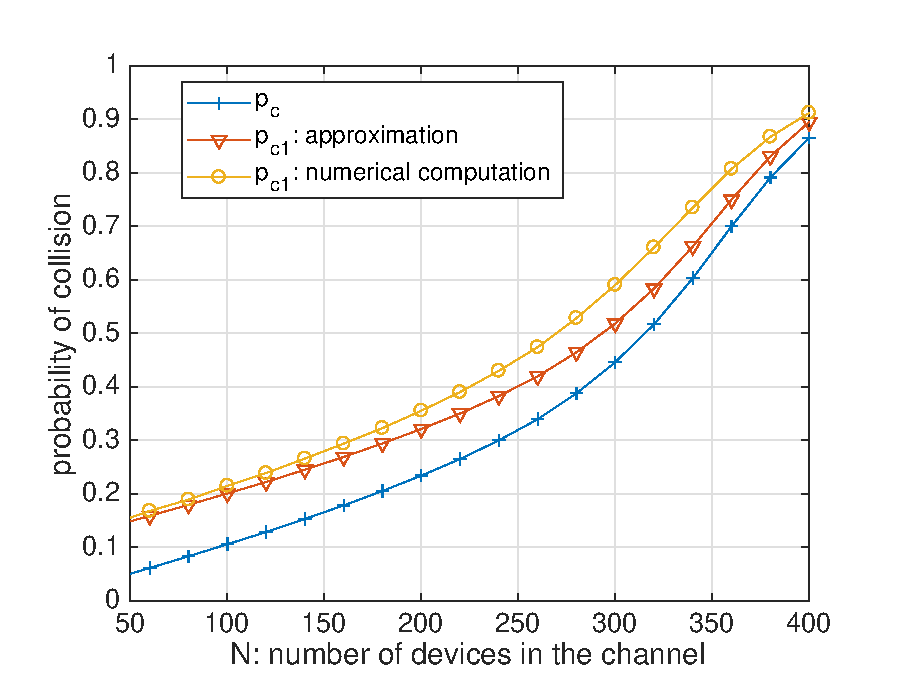
\includegraphics[width=0.65\linewidth]{Approximation_m10.eps}
	\includegraphics[width=0.65\linewidth]{Approximation_m10-eps-converted-to.pdf}
	\caption[Proposed approximation for the probability of collision at the second transmission]{Proposed approximation for the probability of collision at the second transmission. It is more precise for smaller values of $N$.}
	\label{fig:43:Approximation_m10}
\end{figure}


\paragraph{Learning is useful for non-congested networks}

It is worth to highlight that, if we write \eqref{eq:43:decomppc1} as $p_{c1} = p_c + p_{ca} \left(1-p_c\right)$,
then it is obvious that $p_{c1}$ is always larger than $p_c$ (as $p_{ca} \left(1-p_c\right) > 0$).
But for large values of $p_c$, $p_{ca}\left(1-p_c\right) \simeq 0$ so the gap gets small,
and for small values of $p_c$ the gap is significant.
Moreover, we can verify (\eg, numerically or by differentiating)
that the gap decreases when $p_c$ increases (for fixed $N$ and $m$).
This backups mathematically the observation we made from Fig.~\ref{fig:43:Approximation_m10}:
the smaller the $p_c$, the larger is the gap between $p_c$ and $p_{c1}$.

We interpret this fact in two different situations.
\begin{itemize}
	\item
	On the one hand, in a congested network, when devices suffer from a large probability of collision on their first transmission (\ie, $p_c$ is not so small), then $p_{c1}\simeq p_c$ and so devices cannot really hope to reduce their collision probabilities even if the use a different channel for retransmission.
	\item
	On the other hand, if $p_c$ is small enough, \ie, in a network not yet too congested, then our derivation shows that $p_{c1} \gg p_c$, meaning that the possible gain of retransmitting in a different channel that the one used for the first transmission can be large, in terms of collision probability (\eg, up-to $10\%$ in this experimental setting).
	In other words, when learning can be useful (small $p_c$), learning to retransmit in a different channel can have a large impact on the global collision rate,
	thus justifying our approach.
\end{itemize}


\TODOL{Remove this part or compress}

%-----------------------------------------------------------------
\subsection{The \UCB{} algorithm as a building block for different heuristics}
\label{sub:43:MABalgo}
% ----------------------------------------------------------------------

Before presenting our proposed heuristics, we remind here the \UCB{} bandit algorithm \cite{Auer02}.
We include it again to facilitate the understanding of the heuristics, which use \UCB{} as a building block.


% % --- --- --- --- --- --- --- --- --- ---
\paragraph{The \UCB{} algorithm}\label{sub:43:algoUCB}

More formally, for one device, let $N_k(t)$ be the number of times the channel $k$ (for $k\in \llbracket 1, K \rrbracket$) was selected up-to time $t-1$, for $t\geq 0$
for any $t\in\mathbb{N}$,
\begin{equation}\label{eq:43:Nkt}
	N_k(t) = \sum_{\tau=0}^{t-1} \mathbbm{1}(C(\tau) = k),
\end{equation}
The empirical mean estimator $\widehat{\mu_k}(t)$ of channel $k$ is defined as the mean reward obtained up-to time $t-1$,
\begin{equation}\label{eq:43:mukt}
	\widehat{\mu_k}(t) = \frac{1}{N_k(t)} \sum_{\tau=0}^{t-1} r_k(\tau) \mathbbm{1}(C(\tau) = k).
\end{equation}
where $r_{k}(t)$ is the reward obtained after transmission in channel $k$ at time $t$ ($1$ for a successful transmission, and $0$ otherwise)
%
A \emph{confidence} term $B_k(t)$ is given by \cite{Auer02},
\begin{equation}\label{eq:43:Bkt}
	B_k(t) = \sqrt{\alpha \log(t) / N_k(t)},
\end{equation}
where $\alpha$ refers to an exploration coefficient,
% \footnote{~In fact, the larger this coefficient is, the longer the exploration, while the \UCB{} algorithm is proven to be order optimal for $\alpha>0.5$ \cite{Bubeck12}, and has reported a good performance for lower values of $\alpha>0$.},
that we chose equal to $1/2$, as suggested in \cite{Audibert07} and as done in previous works \cite{Bonnefoi18,Bonnefoi17}.
Then, an upper confidence bound in each channel $k$ is defined as
\begin{equation}\label{eq:43:ucb}
	U_k(t) = \widehat{\mu_k}(t) + B_k(t).
\end{equation}
Finally, the transmission channel at time step $t$
is the one maximizing this \UCB{} index $U_k(t)$,
as it is the one expected to be the best one at the current time step $t$,
\begin{equation}\label{eq:43:maxucb}
	C(t) = \arg\max_{1\leq k \leq K} U_k(t).
\end{equation}

The \UCB{} algorithm is implemented independently by each device, and we present it in Algorithm~\ref{algo:43:UCB}.
Note that a device using this first approach is only able to select a channel for the first and all the corresponding retransmissions of a packet.

% \begin{small} % XXX remove if needed
\begin{figure}[h!]
	\centering
	\begin{algorithm}[H]
		% \begin{small} % XXX remove if needed
		\For(){$t = 0, \dots, T$}{
			Compute for each channel $ U_k(t) = \widehat{\mu_k}(t) + B_k(t)$, following Eqs.~\eqref{eq:43:Nkt},~\eqref{eq:43:mukt}, and~\eqref{eq:43:Bkt}\;
			Transmit in channel $C(t) = \arg\max_{1\leq k \leq K} U_k(t)$\;
			Reward $r_{C(t)}(t) = 1$, if \emph{Ack} is received, else $0$\;
		}
		\caption{The \UCB{} algorithm for channel selection (base building block).}
		\label{algo:43:UCB}
		% \end{small} % XXX remove if needed
	\end{algorithm}
\end{figure}
% \end{small} % XXX remove if needed


% ----------------------------------------------------------------------
\subsection{Heuristics to (try to) learn how to retransmit efficiently}
\label{sub:43:heuristics}
% ----------------------------------------------------------------------

A device that implements the UCB algorithm is led to focus is transmissions and retransmissions in the channel which has been identified as the best.
As explained before, focusing in one channel increases the collision probability in retransmissions.
In this Section, we describe the proposed heuristics for the channel selection in a retransmission. It is carried out taking
into account that a device can incorporate a different channel selection strategy while being in a back-off state.
Hence, a natural question is to evaluate whether using this additional contextual information can improve the performance of a learning policy.

For that end, all of our heuristics comprise two stages:
the first stage is a \UCB{} algorithm employed for the first attempt to transmit,
and the second stage is another algorithm used for channel selections for the next retransmissions.
%
We present below four heuristics for this second stage (short names in ``quotes'' correspond to the legend on Figures~\ref{fig:43:mainExperiment1}, \ref{fig:43:mainExperiment2}).


% --- --- --- --- --- --- --- --- --- ---
\paragraph{Uniform random retransmission (``Random'')}\label{sub:43:UCBthenRandom}

In this first proposal, the device uses a random channel selection, following a uniform distribution (in $\llbracket 1, K \rrbracket$).
It is described below in Algorithm~\ref{algo:43:UCBthenRandom}.

\vspace*{-3pt}
\begin{figure}[h!]
	\centering
	\begin{algorithm}[H]
	% \begin{small} % XXX remove if needed
	\For(){$t = 0, \dots, T$}{
			\uIf{First packet transmission}{
				Use first-stage \UCB. %as in Algorithm~\ref{algo:43:UCB}.
			}
			\Else(\tcp*[f]{Random retransmission}){
				Transmit in channel $C(t) \sim \mathcal{U}(1,\ldots,K)$\;
			}
		}
		\caption{Heuristic: uniform random retransmission.}    % A naive
		\label{algo:43:UCBthenRandom}
	% \end{small} % XXX remove if needed
\end{algorithm}
\end{figure}


% --- --- --- --- --- --- --- --- --- ---
\paragraph{\UCB{} for retransmission (``Only \UCB{}'')}\label{sub:43:TwoUCB}

Instead of applying a random channel selection,
another heuristic is to use a second \UCB{} algorithm in the second stage.
In other words, we expect that this algorithm is able to learn the best channel to retransmit a packet.
It is described in Algorithm~\ref{algo:43:TwoUCB}, and it is still a practical approach, since the storage requirements and time complexity remains linear w.r.t. the number of channels $K$ (\ie, of order $\mathcal{O}(K)$).

Note that, we use the subscript $({}^r)$ to denote the variables
$\widehat{\mu^r_k}(t)$, $B^r_k(t)$ and $U^r_k(t)$,
related to the \UCB{} algorithm employed for the retransmission.

\vspace*{-3pt}
% \begin{small} % XXX remove if needed
\begin{figure}[h!]
	\centering
	\begin{algorithm}[H]
		% \begin{small} % XXX remove if needed
		\For(){$t = 0, \dots, T$}{
			\uIf{First packet transmission}{
				Use first-stage \UCB. %as in Algorithm~\ref{algo:43:UCB}.
			}
			\Else(\tcp*[f]{Packet retransmission}){
				Compute for each channel $U^r_k(t) = \widehat{\mu^r_k}(t) + B^r_k(t)$ following Eqs.~\eqref{eq:43:Nkt},~\eqref{eq:43:mukt}, and~\eqref{eq:43:Bkt}\;
				Transmit in channel $C^r(t) = \arg\max_{1\leq k \leq K} U^r_k(t)$\;
				Reward $r^r_{C^r(t)}(t) = 1$, if \emph{Ack} is received, else $0$\;
			}
		}
		\caption{Heuristic: \UCB{} for retransmission.}    % A naive
		\label{algo:43:TwoUCB}
		% \end{small} % XXX remove if needed
		\end{algorithm}
\end{figure}
% \end{small} % XXX remove if needed

% --- --- --- --- --- --- --- --- --- ---
\paragraph{$K$ different {\UCB}s for retransmission (``$K$ \UCB{}'')}\label{sub:43:UCBthenKp1}

Another heuristic is to not use the same algorithm no matter where the collision occurred, but to use $K$ different \UCB{} algorithms.
Meaning that after a failed first transmission in channel $j$, the device relies on the $k$-th algorithm to decide its retransmission.
The corresponding algorithm is depicted in Algorithm~\ref{algo:43:UCBthenKp1}.
Each of these algorithms are denoted using the subscript $({}^{j})$, for $j\in\llbracket 1, K \rrbracket$.

Although, this approach increases the complexity and store requirements (of order $\mathcal{O}(K^2)$).
For our LPWA networks of interest, such as LoRaWAN, the cost of its implementation is still affordable, since a small number of channels is used.
For instance, for $K=4$ channels,
the memory to store $K+1=5$ algorithms is of the order of the requirements to storing one.

Note that for other networks this heuristic could not be practical, for instance Sigfox consist in a large number of very narrow-band channels.
The storage requirements and time complexity is now quadratic in $K$, and as such we no longer consider this heuristic to be a practical proposal in some LPWA networks, as for instance Sigfox networks consist in a large number of very narrow-band channels. But for LoRaWAN networks with $K=4$, storing $K+1=5$ algorithms does not cost much more than storing $2$.

\vspace*{-3pt}
% \begin{small} % XXX remove if needed
	\begin{figure}[h!]
		\centering
		\begin{algorithm}[H]
			% \begin{small} % XXX remove if needed
			% \KwData{$\forall k,j\in[\![1;K]\!]$, $N_k^j(t)$, $\widehat{\mu_k}^j(t)$, $B_k^j(t)$ and $U_k^j(t)$}
			\For(\tcp*[f]{At every time step})
			{$t = 0, \dots, T$}{
				\uIf{First packet transmission}{
					Use first-stage \UCB. %as in Algorithm~\ref{algo:43:UCB}.
				}
				\Else(\tcp*[f]{Packet retransmission}){ % Retr. after trying channel $j$
					j $\leftarrow$ last channel selected by first-stage \UCB\;
					Compute for each channel $U_k^j(t) = \widehat{\mu_k}^j(t) + B_k^j(t)$ following Eqs.~\eqref{eq:43:Nkt},~\eqref{eq:43:mukt}, and~\eqref{eq:43:Bkt}\;
					Transmit in channel $C^j(t) = \arg\max_{1\leq k \leq K} U^j_k(t)$\;
					Reward $r^j_{C^j(t)}(t) = 1$ if \emph{Ack} is received, else $0$\;
				}
			}
			\caption{Heuristic: $K$ different {\UCB}s for retransmission.}
			\label{algo:43:UCBthenKp1}
			% \end{small} % XXX remove if needed
		\end{algorithm}
	\end{figure}
% \end{small} % XXX remove if needed

% --- --- --- --- --- --- --- --- --- ---
\paragraph{Delayed \UCB{} for retransmission (``Delayed \UCB{}'')}\label{sub:43:UCBwithDelay}

This last heuristic is a composite of
the random retransmission (Algorithm~\ref{algo:43:UCBthenRandom})
and the \UCB{} retransmission (Algorithm~\ref{algo:43:TwoUCB}) approaches.
Instead of starting the second stage \UCB{} directly from the first retransmission, we introduce a fixed delay $\Delta\in\mathbb{N}$, $\Delta \geq 1$,
and start to rely on the second stage \UCB{} after $\Delta$ transmissions.
The selection for the first steps is handled with the random retransmission.

The idea behind this delay is to allow the first stage \UCB{} to start learning the best channel, before starting the second stage \UCB{} (see details in Algorithm~\ref{algo:43:UCBwithDelay}).
The number of transmissions to wait before applying the second algorithm is denoted by $\Delta$, it has to be fixed before-hand\footnote{~Choosing the value of $\Delta$ could be done by extensive benchmarks but such approach goes against the reinforcement learning idea: an heuristic should work against any problem, without the need to be able to simulate the problem in advance in order to find a good value of some internal parameter. As such, we only consider a delay of $\Delta=100$.}.

Note that, we use the subscript $({}^d)$ to denote the variables
related to the delayed second-stage \UCB{} algorithm.

\vspace*{-3pt}
% \begin{small} % XXX remove if needed
	\begin{figure}[h!]
		\centering
		\begin{algorithm}[H]
			% \begin{small} % XXX remove if needed
			\For(\tcp*[f]{At every time step})
			{$t = 0, \dots, T$}{
				\uIf{First packet transmission}{
			 		Use first-stage \UCB. %as in Algorithm~\ref{algo:43:UCB}.
				}
				\uElseIf(\tcp*[f]{Random retransmission}){$t \leq \Delta$}{
					Transmit randomly in a channel $C(t) \sim \mathcal{U}(1,\ldots,K)$.
				}
				\Else(\tcp*[f]{Delayed \UCB{}}){
					Compute for each channel $ U^d_k(t) = \widehat{\mu^d_k}(t) + B^d_k(t)$ following Eqs.~\eqref{eq:43:Nkt},~\eqref{eq:43:mukt}, and~\eqref{eq:43:Bkt}\;
					Transmit in channel $C^d(t) = \arg\max_{1\leq k \leq K} U^d_k(t)$\;
					Reward $r^d_{C^d(t)}(t) = 1$ if \emph{Ack} is received, else $0$\;
				}
			}
			\caption{Heuristic: Delayed \UCB{} for retransmission.}
			\label{algo:43:UCBwithDelay}
			% \end{small} % XXX remove if needed
		\end{algorithm}
	\end{figure}
% \end{small} % XXX remove if needed


% ----------------------------------------------------------------------
\subsection{Simulations to compare our heuristics}
\label{sub:43:numExp}
% ----------------------------------------------------------------------

We simulate our network considering $N$ devices following the contention Markov process described in Section \ref{sub:43:model}, and a LoRa standard with $K=4$ channels.
Each device is set to transmit with a fixed probability $p=10^{-3}$, \ie, a packet about every $20$ minutes for time slots of $1\;\mathrm{s}$.
%
For the evaluation of the proposed heuristics, a total number of $T=10^{6}$ time slots is considered, and the results are averaged over $10^{3}$ independent random simulations.
%In this way, it allows us to evaluate the learning rate, as well as the convergence of each learning approach.

In a first scenario, we consider a total number of $N=1000$ IoT devices, with a non-uniform repartition of static devices given by $10\%,30\%,30\%,30\%$ for the four channels.
In other words, the channels are occupied $10\%$, $30\%$, $30\%$, and $30\%$ of time, and the contention Markov process considered is given by $M = 5$, and $m=5$.
In Fig.~\ref{fig:43:mainExperiment1}, we show the successful transmission rate versus the number of slots, for all the proposed heuristics.

A first result is that all the heuristics clearly outperform the non-learning approach that simply use random channel selection for both transmissions and retransmissions (\ie, the \textbf{no \UCB{}} curve).
The improvement of the heuristics over the non-learning approach is evident, and for every heuristic that use a kind of learning mechanism it can observed a successful transmission rate that increases rapidly (or equivalently an PLR decreasing).
Moreover, all of these approaches show a fast convergence making them suitable for the targeted application.
It is also worths mentioning that the employment of the same \UCB{} algorithm for retransmissions denoted here as ``Only \UCB{}'' achieves a better performance, while a ``Random" retransmission features a slight degradation. This result can be explained as follows: the loss of performance related to the separation of information for several algorithms is greater than the gain obtained by considering the first transmissions and retransmissions separately.

\begin{figure}[h!]  % [htbp]
	\centering
	\includegraphics[width=0.75\linewidth]{ResultsUCB.eps}
	\caption[First comparison between the exposed heuristics for the retransmission: Only \UCB, Random, \UCB, $K$ \UCB, and Delayed \UCB]{
		Comparison between the exposed heuristics for the retransmission: \textcolor{blue}{Only \UCB}, \textcolor{cyan}{Random}, \textcolor{purple}{\UCB}, \textcolor{green}{$K$ \UCB}, and \textcolor{red}{Delayed \UCB}.
		The usage of the same learning policy for transmissions and retransmission is named \textcolor{blue}{Only \UCB{}},
		whereas the usage of a random channel selection, for both transmission and retransmission, is labeled as \textbf{no \UCB{}}.
		First scenario: learning helps but learning to retransmit smartly is not needed, as we observe that the \textcolor{cyan}{random retransmission} heuristic achieves similar performance than the others.
	}
	\label{fig:43:mainExperiment1}
\end{figure}

We also consider in our analysis the case where $M=5$, and $m=10$ using ALOHA protocol, a statistic distribution of the devices about $40\%, 30\%, 20\%, 10\%$ for the four channels, and $N=2000$ IoT devices.
The corresponding results are depicted in Fig.~\ref{fig:43:mainExperiment2}.
In this case the successful transmission rate is degraded compared with achieved results in Fig.~\ref{fig:43:mainExperiment1}, this can be explained with the fact that we are considering in our network more devices that increase the collision probability.
It is important to highlight,that the ``Random" retransmission heuristic shows a poor performance in comparison to the other heuristics, and it can be attributed to the fact that the number of retransmission is increased, and consequently a
learning approach is able to take advantage of it.
Furthermore, the ``Delayed \UCB'' and  the``\UCB'' heuristics show quite similar results, after converging.
%
%Random, \UCB{}, $K$ \UCB{}, Delayed \UCB{} obtain similar results. The less efficient one is the $K$ \UCB{}, and this makes sense as having more learning algorithm needs more for each of them to learn. The most efficient one is the simple \UCB{} procedure, and this was quite surprising.

\begin{figure}[h!]  % [htbp]
	\centering
	\includegraphics[width=0.75\linewidth]{ResultsUCB2.eps}
	\caption[First comparison between the exposed heuristics for the retransmission: Only \UCB, Random, \UCB, $K$ \UCB, and Delayed \UCB]{
		Second scenario: learning helps a lot (a gain of $30\%$ in terms of collision probability), and learning to retransmit smartly is needed.
		We observe that the \textcolor{cyan}{random retransmission} achieves poor performance compared to the others.
	}
	\label{fig:43:mainExperiment2}
\end{figure}

The conclusions we can draw from depicted results are twofold.
First, MAB learning algorithms are very useful to reduce the collision rate in LPWA networks, a gain of up-to $30\%$ of successful transmission rate is observed after convergence.
A second conclusion that can be highlighted is that, using learning mechanisms for retransmissions can be an interesting way to reduce collisions in networks with massive deployments of IoT as this can be checked in Fig.~\ref{fig:43:mainExperiment2}, where the random retransmission heuristic is not very advantageous in front of the  \UCB-based approaches that use learning for channel selection during the retransmission procedure.


\paragraph{Note on the simulation code}
%
The source code (MATLAB or Octave) used for the simulations and the figures of this Section is open-sourced under the MIT License, and published at \href{https://Bitbucket.org/scee_ietr/ucb_smart_retrans}{\texttt{Bitbucket.org/scee\_ietr/ucb\_smart\_retrans}}.
It was written in collaboration with Rémi Bonnefoi and Julio César Mango-Vasquez, in July and August $2018$.



% ----------------------------------------------------------------------------
\section{Conclusion of Chapter~\ref{chapter:4}}
\label{sec:4:conclusion}
% ----------------------------------------------------------------------

We give in this Section conclusions about the two models presented above and about our demonstration, as well as many directions of future works, some of which are currently being studied by researchers of our team.


% ----------------------------------------------------------------------
\paragraph{Summary of the first model}
\label{sub:41:conclusion}

In Section~\ref{sec:4:firstModel}, we proposed an evaluation of the performance of MAB learning algorithms in IoT networks,
with a focus on the convergence of algorithms, in terms of successful transmission rates, when the proportion of intelligent dynamic devices changes.
Concretely, increasing this probability allows to insert more objects in the same network, while maintaining a good Quality of Service.
We show that \UCB{} and TS have near-optimal performance, even when their underlying \iid{} assumption is violated by the many ``intelligent'' end-devices.

This is both a surprising and a very encouraging result, showing that application of bandit algorithms tailored for a stochastic model is still useful in broader settings.
The fully \emph{decentralized} application of classic stochastic MAB algorithms are almost as efficient as the best possible centralized policy in this setting, after a short learning period, even though the dynamic devices \emph{can not} communicate with each others, and \emph{do not} know the system parameters.
We will investigate this behavior in order to understand it better theoretically.
We will also experiment more with adversarial algorithms, to confirm that they work less efficiently than stochastic bandit algorithms in our non-stochastic setting.


% ----------------------------------------------------------------------
\paragraph{Conclusions taken from the demonstration}
\label{sub:42:conclusionFromDemonstration}

We presented in Section~\ref{sec:4:gnuradio} a demonstration, showed in $2018$ at the ICT conference \cite{Besson2018ICT}, and further detailed in the companion paper \cite{Besson2019WCNC}.
We gave all the necessary details on both the PHY and the MAC layer, as well as details on the User Interface developed for the demo.
Results obtained in practice were discussed, to highlight the interest of using learning algorithms for radio online optimization problem, and especially multi-armed bandit learning algorithms.
%
By using such low-cost algorithms, we demonstrated empirically that a dynamically reconfigurable object can learn on its own to favor a certain channel, if the environment traffic is not uniform between the $K$ different channels.


% ----------------------------------------------------------------------
\paragraph{Conclusion about this second model}
\label{sub:43:conclusion}

In Section~\ref{sec:4:retransmissions}, we presented an extension of our model of LPWA networks based on an ALOHA protocol, slotted both in time and frequency, in which dynamic IoT devices can use machine learning algorithms, to improve their Packet Loss Ratio (PLR) when accessing the network.
The main novelty of this model is to address the packet retransmissions upon radio collision, by using a Multi-Armed Bandit framework.
We presented and evaluated several learning heuristic that try to learn how to transmit and retransmit in a smarter way, by using the \UCB{} algorithm for channel selection for first transmission, and different proposals based on \UCB{} for the retransmissions upon collisions.

We showed that incorporating learning for the transmission is needed to achieve optimal performance, with significant gain in terms of successful transmission rate in networks with a large number of devices (up-to $30\%$ in the example network).
Our empirical simulations show that each of our proposed heuristic outperforms a naive random access scheme.
Surprisingly, the main take-away message is that a simple \UCB{} learning approach, that retransmit in the same channel, turns out to perform as well as more complicated heuristics.


% ----------------------------------------------------------------------
\paragraph{Future works}
\label{sub:4:futureWorks}

Future works related to this Chapter include the following directions.


\paragraph{Possible extensions of the first model}

The first model presented in Section~\ref{sec:4:firstModel} could easily be generalized with two probabilities $p_S$ and $p_D$, if static and dynamic devices had different transmission pattern, and less easily with one probability per device. Also, other emission pattern could be considered, instead of a Bernoulli process for each user.
We prefer to consider that all devices have the same probability to transmit to keep the notation as simple as possible.

Moreover, for sake of simplicity we supposed that all devices use the same standard. Our future work will consider more realistic interference scenarios and IoT networks, with, \emph{e.g.}, non-slotted time, more than one base station etc.

Another extension could be to not have a Bernoulli process (or any random process), but a fixed rate of transmission, \emph{e.g.}, one transmission a day.
So additionally to deciding the channel for communication, each device has to also decide when to communicate.
This is another direction of research, that we will investigate in the future.

\paragraph{Extensions of the demonstration}

Possible future extensions of our demonstration include the following points.
We could consider more dynamic objects (\emph{e.g.}, $100$) but it would either cost more in terms of equipment, or in terms of software engineering to simulation more objects with the same card.
We could also implement a real-world IoT communication protocol (like the LoRaWAN standard), which we prefer not to do as it would cost a significant effort of development.
Finally, we could also study the interference in case of other gateways located nearby, and this could be done without needing new hardware.
%
% Pub pour notre autre article
% We are also interested in studying the possible gain of using a learning step when the transmission model follows ALOHA-like retransmissions, and this is presented in the next Section~\ref{sec:4:retransmissions}.


\paragraph{Possible extensions for the second model}

The utility and impact of the proposed approaches for LPWA networks motivates us to address several subjects as future works. Among them, the non-stationarity of the channel occupancy caused by the learning policy employed by the IoT devices.
%
For that end, modifications of MAB algorithms have been proposed, such as Sliding-Window-\UCB{} or Discounted-\UCB{} \cite{Garivier11UCBDiscount}
or more recently M-\UCB{} \cite{CaoZhenKvetonXie18},
or more recently GLR-\UCB{} \cite{Besson2019GLRT} which is presented in Chapter~\ref{chapter:6},
that nevertheless have not been explored for the targeted problem.
Chapter~\ref{chapter:6} is focusing on this direction, but we did not have enough time to explore the possible applications of MAB policies designed for non-stationary problems to the model with retransmissions presented in this section.

In order to validate our results in a realistic experimental setting and not only with simulations, future works include a hardware implementation of the analyzed models to complete our demonstration \cite{Besson2019WCNC}.
Note that Julio César Mango-Vasquez is currently working on this direction, for the EPHYL project, in collaboration with Carlos Faouzi Bader at IETR and CentraleSupélec campus of Rennes, and Christophe Moy at IETR and University Rennes 1.
%
A hardware demonstrator could be also benefit to study other settings by removing some hypotheses, for instance by studying a similar model in non-slotted time.


% ----------------------------------------------------------------------------
\section{Appendix for Chapter~\ref{chapter:4}}
\label{sec:4:appendix}
% ----------------------------------------------------------------------------

We include here a missing proof from Section~\ref{sec:4:firstModel}.

% \subsection{Proof of Proposition \ref{prop:41:Lagrangian}}
% \label{sec:5:proofLagrangian}

This short subsection contains the missing details of the proof of Proposition \ref{prop:41:Lagrangian}.
%
First, we need to justify that the objective function is quasi-convex, in each of its coordinates.
%
Then, we develop the computation of $D_i^*(\lambda)$, as a closed form expression of the system parameters ($K, p$), the repartition of static devices ($S_1,\dots,S_{K}$) and the Lagrange multiplier $\lambda$.

\paragraph{Quasi-convexity}

\begin{itemize}
	\item
	For $0 < \gamma < 1$, the function: $g: x \mapsto x \gamma^x$ is quasi-convex on $[0,\infty)$, \ie, $g(\eta x + (1-\eta)y) \leq \max(g(x), g(y))$ for any $x,y \in [0,\infty)$ and $\eta \in [0,1]$ (definition from \cite{Luenberger68}).
    Indeed, $g(\eta x + (1-\eta)y) = \eta \left[ x (\gamma^x)^{\eta} \right] \gamma^{((1-\eta)y)} + (1-\eta)\left[ y (\gamma^y)^{1-\eta}\right] \gamma^{\eta x}$, and $\gamma^{((1-\eta)y)} \leq 1$ and $\gamma^{\eta x} \leq 1$. But also $(\gamma^x)^{\eta} \leq \gamma^x$ as $\eta \leq 1$, and the same holds for $(\gamma^y)^{1-\eta} \leq \gamma^y$. So $g(\eta x + (1-\eta)y) \leq \eta (x \gamma^x) + (1 - \eta) (y \gamma^y)$ which is a convex combination of $x \gamma^x$ and $y \gamma^y$, so smaller than the larger of the two values, and so $g(\eta x + (1-\eta)y) \leq \max(x \gamma^x, y \gamma^y)$.

    \item
    The function $f: (D_1, \dots, D_{K}) \mapsto \sum_{i=1}^{K} D_i (1 - p)^{S_i + D_i -1}$ is quasi-convex in each of its coordinates, on $[0,\infty)^{K}$, as a sum of component-wise quasi-convex functions (with $\gamma = (1 - p) \in (0, 1)$, thanks to the first point).
    \hfill{}$\square$
\end{itemize}


\paragraph{Derivation of the Lagrange multiplier solution}

Let us now prove the expression for $D_i^*$ given in \eqref{eq:41:Dilambda}.
\begin{itemize}
	\item
	If $\boldsymbol{D} = (D_1,\dots,D_{K})$,
    the Lagrangian is denoted $\mathcal{L}(\boldsymbol{D}, \lambda) = f(\boldsymbol{D}) + \lambda(D - \sum_{i=1}^{K} D_i)$, and its derivative w.r.t. $D_i$ is
    $\frac{\partial}{\partial D_i} \mathcal{L}(\boldsymbol{D}, \lambda) = (1-p)^{S_i + D_i - 1} + \log(1 - p) D_i (1-p)^{S_i + D_i - 1} - \lambda$.

    \item
    So the gradient is zero $\frac{\partial}{\partial D_i} \mathcal{L}(\boldsymbol{D}, \lambda) |_{D_i=D_i^*} = 0$
    iff $D_i^*$ satisfies $(1-p)^{D_i^*}( 1 + \log(1-p) D_i^*) = \lambda / (1-p)^{S_i - 1}$. Let $x = \log(1-p) D_i^*$ this is equivalent to $\mathrm{e}^{x}(1 + x) = \lambda / (1-p)^{S_i - 1}$
    and with $y = 1 + x$, we get $\mathrm{e}^{y}y = \lambda\mathrm{e} / (1-p)^{S_i - 1}$.

	\item
    By using the $\mathcal{W}$-Lambert function $\mathcal{W}$ \cite{Corless96}, reciprocal of $y \mapsto \mathrm{e}^{y}y$, we get $x = y - 1 = \mathcal{W}(\lambda\mathrm{e} / (1-p)^{S_i - 1}) - 1$.
    So the gradient of the Lagrangian is zero iff $D_i^* = \max(0, 1/\log(1-p) x) = \left[ \frac{1}{\log(1-p)}\mathcal{W}(\lambda\mathrm{e} / (1-p)^{S_i - 1}) - 1\right]^{+}$, because $D_i^*$ has to be non-negative.
    This gives the $i$-th coordinate of the unique saddle point of $f(\boldsymbol{D})$,
    and so the unique solution to the maximization problem \eqref{eq:41:optPb}, thanks to \cite[Theorem 1]{Luenberger68}.
    \hfill{}$\square$
\end{itemize}


